\documentclass[aspectratio=169]{beamer}
\IfFileExists{beamerthememetropolis.sty}{\usetheme{metropolis}}{\usetheme{default}}
\usepackage[utf8]{inputenc}
\usepackage[T1]{fontenc}
\usepackage{booktabs}
\usepackage{graphicx}
\usepackage{amsmath}
\usepackage{xcolor}
\usepackage{tikz}
\definecolor{shipblue}{RGB}{20,74,130}
\definecolor{warningorange}{RGB}{210,105,30}
\setbeamercolor{structure}{fg=shipblue}
\setbeamercolor{alerted text}{fg=warningorange}
\setbeamertemplate{navigation symbols}{}
\title{EXEC\_10: EndTop photon budget and intrinsic timing}
\subtitle{Landau-dominated Npe, clarified timing densities, and apparent-slope diagnosis}
\author{Rene Rios (ULS)}
\date{June 11, 2026}
\begin{document}
\begin{frame}{Configuration and provenance}

\begin{columns}[T]\column{0.62\textwidth}
\textbf{Branch:} \texttt{feat/endtop-sslg4}\\
\textbf{Commits:} \texttt{0201413}, \texttt{7b4bc80}, \texttt{ad26d78},
\texttt{bcefa24}, \texttt{bdfe955}; this deck is generated from those published sources
\begin{itemize}\small
  \item 31 positions $\times$ 2000 events; 16 End + 70 Top channels; jitter fixed to zero.
  \item EJ-204 via SSLG4 \texttt{OPSC-101}: yield 10400/MeV, $\tau_r=0.7$ ns,
        $\tau_d=1.8$ ns, ABSLENGTH=160 cm (verified effective MPT inputs).
  \item Broadcom AFBR-S4N66P024M: PDE 63\% at 420 nm.
\end{itemize}
\column{0.35\textwidth}
\begin{alertblock}{Scope}
Top 70 SiPM is a simulation coverage study. Real hardware: 32 Top SiPMs.
All reported timing is intrinsic, without SPTR or electronics jitter.
\end{alertblock}
\end{columns}

\end{frame}
\begin{frame}{EndTop geometry and channel map}

\begin{columns}[T]\column{0.55\textwidth}
\begin{itemize}
 \item EJ-204 bar: $1400\times60\times10$ mm$^3$.
 \item End L IDs 0--7; End R IDs 8--15.
 \item Top L IDs 16--50: $-692,-672,\ldots,-12$ mm.
 \item Top R IDs 51--85: $+12,+32,\ldots,+692$ mm.
 \item Each Top element and window: $6\times6$ mm$^2$.
\end{itemize}
\column{0.42\textwidth}
\begin{block}{Exact constraints}
First centers are 5 mm from each bar end. Pitch is 20 mm except the deliberate
central $-12/+12$ mm pair, whose pitch is 24 mm.
\end{block}
\end{columns}

\end{frame}
\begin{frame}{Instrumented and wrapped faces}

\centering\begin{tabular}{lll}\toprule
Face & Optical state & Readout \\ \midrule
$-X$, $+X$ & open & 8 End SiPMs each \\
$+Y$ & Mylar with 70 exact windows & 70 Top SiPMs \\
$-Y$, $-Z$, $+Z$ & complete Mylar & none \\
\bottomrule\end{tabular}
\vspace{0.5cm}
\begin{block}{External layer}
Black Tedlar is deliberately not modeled; it only blocks ambient light.
The non-reflected Mylar fraction is already absorbed in the optical model.
\end{block}

\end{frame}
\begin{frame}{Window optics: why timing and collection change}

\centering
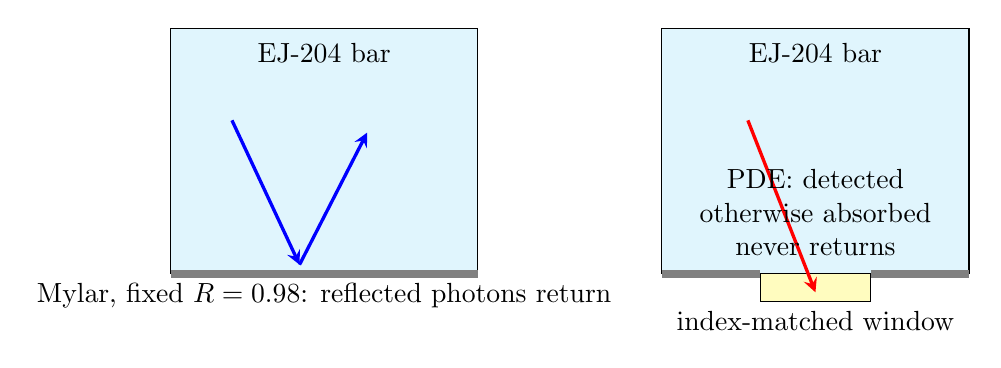
\begin{tikzpicture}[scale=0.78,>=stealth]
 \draw[fill=cyan!12] (0,0) rectangle (5,4);
 \node at (2.5,3.6) {EJ-204 bar};
 \draw[line width=3pt,gray] (0,0) -- (5,0);
 \node[below] at (2.5,0) {Mylar, fixed $R=0.98$: reflected photons return};
 \draw[->,very thick,blue] (1.0,2.5) -- (2.1,0.15);
 \draw[->,very thick,blue] (2.1,0.15) -- (3.2,2.3);
 \draw[fill=cyan!12] (8,0) rectangle (13,4);
 \node at (10.5,3.6) {EJ-204 bar};
 \draw[line width=3pt,gray] (8,0) -- (9.6,0);
 \draw[line width=3pt,gray] (11.4,0) -- (13,0);
 \draw[fill=yellow!25] (9.6,-0.45) rectangle (11.4,0);
 \node[below] at (10.5,-0.45) {index-matched window};
 \draw[->,very thick,red] (9.4,2.5) -- (10.5,-0.3);
 \node[align=center] at (10.5,1.0) {PDE: detected\\otherwise absorbed\\never returns};
\end{tikzpicture}
\begin{alertblock}{Consequence}
Every window is an optical drain. Long, multiply reflected paths have more chances
to meet one, so late End photons are preferentially removed.
\end{alertblock}

\end{frame}
\section{Position-by-position}
\begin{frame}{Position x=-690 mm}

\begin{columns}[T]
  \column{0.52\textwidth}
  
\includegraphics[width=\textwidth]{figs/muon_-690mm_geometry.png}
  \column{0.46\textwidth}
  
\includegraphics[width=\textwidth]{figs/muon_-690mm_top_profile.png}
  \tiny
  \begin{tabular}{lr}
    \toprule Quantity & Value \\ \midrule
    End L $N_{pe}$ & $3363.1\pm18.1$ \\
    End R $N_{pe}$ & $41.1\pm0.3$ \\
    Nearest Top ID & 16 (window-track exception) \\
    Nearest Top $N_{pe}$ & $350.9\pm2.0$ \\
    Nearest Top $\langle t\rangle$ &
      $2.7863\pm0.0023$ ns \\
    Nearest Top FPT & $0.34278\pm0.00023$ ns \\
    \bottomrule
  \end{tabular}
\end{columns}

\end{frame}
\begin{frame}{Position x=-670 mm}

\begin{columns}[T]
  \column{0.52\textwidth}
  
\includegraphics[width=\textwidth]{figs/muon_-670mm_geometry.png}
  \column{0.46\textwidth}
  
\includegraphics[width=\textwidth]{figs/muon_-670mm_top_profile.png}
  \tiny
  \begin{tabular}{lr}
    \toprule Quantity & Value \\ \midrule
    End L $N_{pe}$ & $2764.3\pm15.0$ \\
    End R $N_{pe}$ & $42.6\pm0.3$ \\
    Nearest Top ID & 17 (window-track exception) \\
    Nearest Top $N_{pe}$ & $350.4\pm2.0$ \\
    Nearest Top $\langle t\rangle$ &
      $2.7753\pm0.0023$ ns \\
    Nearest Top FPT & $0.34261\pm0.00021$ ns \\
    \bottomrule
  \end{tabular}
\end{columns}

\end{frame}
\begin{frame}{Position x=-650 mm}

\begin{columns}[T]
  \column{0.52\textwidth}
  
\includegraphics[width=\textwidth]{figs/muon_-650mm_geometry.png}
  \column{0.46\textwidth}
  
\includegraphics[width=\textwidth]{figs/muon_-650mm_top_profile.png}
  \tiny
  \begin{tabular}{lr}
    \toprule Quantity & Value \\ \midrule
    End L $N_{pe}$ & $2366.2\pm13.1$ \\
    End R $N_{pe}$ & $44.3\pm0.3$ \\
    Nearest Top ID & 18 (window-track exception) \\
    Nearest Top $N_{pe}$ & $351.0\pm2.0$ \\
    Nearest Top $\langle t\rangle$ &
      $2.7779\pm0.0023$ ns \\
    Nearest Top FPT & $0.34270\pm0.00024$ ns \\
    \bottomrule
  \end{tabular}
\end{columns}

\end{frame}
\begin{frame}{Position x=-600 mm}

\begin{columns}[T]
  \column{0.52\textwidth}
  
\includegraphics[width=\textwidth]{figs/muon_-600mm_geometry.png}
  \column{0.46\textwidth}
  
\includegraphics[width=\textwidth]{figs/muon_-600mm_top_profile.png}
  \tiny
  \begin{tabular}{lr}
    \toprule Quantity & Value \\ \midrule
    End L $N_{pe}$ & $1673.6\pm9.2$ \\
    End R $N_{pe}$ & $48.0\pm0.3$ \\
    Nearest Top ID & 21 (exact geometry) \\
    Nearest Top $N_{pe}$ & $408.0\pm2.2$ \\
    Nearest Top $\langle t\rangle$ &
      $2.9421\pm0.0022$ ns \\
    Nearest Top FPT & $0.34610\pm0.00021$ ns \\
    \bottomrule
  \end{tabular}
\end{columns}

\end{frame}
\begin{frame}{Position x=-550 mm}

\begin{columns}[T]
  \column{0.52\textwidth}
  
\includegraphics[width=\textwidth]{figs/muon_-550mm_geometry.png}
  \column{0.46\textwidth}
  
\includegraphics[width=\textwidth]{figs/muon_-550mm_top_profile.png}
  \tiny
  \begin{tabular}{lr}
    \toprule Quantity & Value \\ \midrule
    End L $N_{pe}$ & $1323.9\pm7.6$ \\
    End R $N_{pe}$ & $55.1\pm0.4$ \\
    Nearest Top ID & 23 (window-track exception) \\
    Nearest Top $N_{pe}$ & $352.9\pm2.1$ \\
    Nearest Top $\langle t\rangle$ &
      $2.7760\pm0.0023$ ns \\
    Nearest Top FPT & $0.34276\pm0.00025$ ns \\
    \bottomrule
  \end{tabular}
\end{columns}

\end{frame}
\begin{frame}{Position x=-500 mm}

\begin{columns}[T]
  \column{0.52\textwidth}
  
\includegraphics[width=\textwidth]{figs/muon_-500mm_geometry.png}
  \column{0.46\textwidth}
  
\includegraphics[width=\textwidth]{figs/muon_-500mm_top_profile.png}
  \tiny
  \begin{tabular}{lr}
    \toprule Quantity & Value \\ \midrule
    End L $N_{pe}$ & $1042.2\pm5.9$ \\
    End R $N_{pe}$ & $59.8\pm0.4$ \\
    Nearest Top ID & 26 (exact geometry) \\
    Nearest Top $N_{pe}$ & $410.9\pm2.3$ \\
    Nearest Top $\langle t\rangle$ &
      $2.9419\pm0.0022$ ns \\
    Nearest Top FPT & $0.34607\pm0.00023$ ns \\
    \bottomrule
  \end{tabular}
\end{columns}

\end{frame}
\begin{frame}{Position x=-450 mm}

\begin{columns}[T]
  \column{0.52\textwidth}
  
\includegraphics[width=\textwidth]{figs/muon_-450mm_geometry.png}
  \column{0.46\textwidth}
  
\includegraphics[width=\textwidth]{figs/muon_-450mm_top_profile.png}
  \tiny
  \begin{tabular}{lr}
    \toprule Quantity & Value \\ \midrule
    End L $N_{pe}$ & $832.9\pm4.2$ \\
    End R $N_{pe}$ & $65.8\pm0.4$ \\
    Nearest Top ID & 28 (window-track exception) \\
    Nearest Top $N_{pe}$ & $345.8\pm1.8$ \\
    Nearest Top $\langle t\rangle$ &
      $2.7793\pm0.0023$ ns \\
    Nearest Top FPT & $0.34237\pm0.00016$ ns \\
    \bottomrule
  \end{tabular}
\end{columns}

\end{frame}
\begin{frame}{Position x=-400 mm}

\begin{columns}[T]
  \column{0.52\textwidth}
  
\includegraphics[width=\textwidth]{figs/muon_-400mm_geometry.png}
  \column{0.46\textwidth}
  
\includegraphics[width=\textwidth]{figs/muon_-400mm_top_profile.png}
  \tiny
  \begin{tabular}{lr}
    \toprule Quantity & Value \\ \midrule
    End L $N_{pe}$ & $691.3\pm3.9$ \\
    End R $N_{pe}$ & $74.5\pm0.5$ \\
    Nearest Top ID & 31 (exact geometry) \\
    Nearest Top $N_{pe}$ & $411.3\pm2.3$ \\
    Nearest Top $\langle t\rangle$ &
      $2.9399\pm0.0022$ ns \\
    Nearest Top FPT & $0.34597\pm0.00021$ ns \\
    \bottomrule
  \end{tabular}
\end{columns}

\end{frame}
\begin{frame}{Position x=-350 mm}

\begin{columns}[T]
  \column{0.52\textwidth}
  
\includegraphics[width=\textwidth]{figs/muon_-350mm_geometry.png}
  \column{0.46\textwidth}
  
\includegraphics[width=\textwidth]{figs/muon_-350mm_top_profile.png}
  \tiny
  \begin{tabular}{lr}
    \toprule Quantity & Value \\ \midrule
    End L $N_{pe}$ & $575.0\pm3.1$ \\
    End R $N_{pe}$ & $84.1\pm0.5$ \\
    Nearest Top ID & 33 (window-track exception) \\
    Nearest Top $N_{pe}$ & $349.3\pm1.9$ \\
    Nearest Top $\langle t\rangle$ &
      $2.7748\pm0.0023$ ns \\
    Nearest Top FPT & $0.34234\pm0.00015$ ns \\
    \bottomrule
  \end{tabular}
\end{columns}

\end{frame}
\begin{frame}{Position x=-300 mm}

\begin{columns}[T]
  \column{0.52\textwidth}
  
\includegraphics[width=\textwidth]{figs/muon_-300mm_geometry.png}
  \column{0.46\textwidth}
  
\includegraphics[width=\textwidth]{figs/muon_-300mm_top_profile.png}
  \tiny
  \begin{tabular}{lr}
    \toprule Quantity & Value \\ \midrule
    End L $N_{pe}$ & $482.3\pm2.8$ \\
    End R $N_{pe}$ & $94.2\pm0.6$ \\
    Nearest Top ID & 36 (exact geometry) \\
    Nearest Top $N_{pe}$ & $413.7\pm2.5$ \\
    Nearest Top $\langle t\rangle$ &
      $2.9387\pm0.0022$ ns \\
    Nearest Top FPT & $0.34593\pm0.00023$ ns \\
    \bottomrule
  \end{tabular}
\end{columns}

\end{frame}
\begin{frame}{Position x=-250 mm}

\begin{columns}[T]
  \column{0.52\textwidth}
  
\includegraphics[width=\textwidth]{figs/muon_-250mm_geometry.png}
  \column{0.46\textwidth}
  
\includegraphics[width=\textwidth]{figs/muon_-250mm_top_profile.png}
  \tiny
  \begin{tabular}{lr}
    \toprule Quantity & Value \\ \midrule
    End L $N_{pe}$ & $415.8\pm2.4$ \\
    End R $N_{pe}$ & $105.5\pm0.7$ \\
    Nearest Top ID & 38 (window-track exception) \\
    Nearest Top $N_{pe}$ & $352.2\pm2.1$ \\
    Nearest Top $\langle t\rangle$ &
      $2.7758\pm0.0023$ ns \\
    Nearest Top FPT & $0.34224\pm0.00013$ ns \\
    \bottomrule
  \end{tabular}
\end{columns}

\end{frame}
\begin{frame}{Position x=-200 mm}

\begin{columns}[T]
  \column{0.52\textwidth}
  
\includegraphics[width=\textwidth]{figs/muon_-200mm_geometry.png}
  \column{0.46\textwidth}
  
\includegraphics[width=\textwidth]{figs/muon_-200mm_top_profile.png}
  \tiny
  \begin{tabular}{lr}
    \toprule Quantity & Value \\ \midrule
    End L $N_{pe}$ & $353.5\pm2.0$ \\
    End R $N_{pe}$ & $118.4\pm0.7$ \\
    Nearest Top ID & 41 (exact geometry) \\
    Nearest Top $N_{pe}$ & $412.5\pm2.3$ \\
    Nearest Top $\langle t\rangle$ &
      $2.9407\pm0.0022$ ns \\
    Nearest Top FPT & $0.34577\pm0.00020$ ns \\
    \bottomrule
  \end{tabular}
\end{columns}

\end{frame}
\begin{frame}{Position x=-150 mm}

\begin{columns}[T]
  \column{0.52\textwidth}
  
\includegraphics[width=\textwidth]{figs/muon_-150mm_geometry.png}
  \column{0.46\textwidth}
  
\includegraphics[width=\textwidth]{figs/muon_-150mm_top_profile.png}
  \tiny
  \begin{tabular}{lr}
    \toprule Quantity & Value \\ \midrule
    End L $N_{pe}$ & $302.1\pm1.8$ \\
    End R $N_{pe}$ & $134.7\pm0.8$ \\
    Nearest Top ID & 43 (window-track exception) \\
    Nearest Top $N_{pe}$ & $350.8\pm2.1$ \\
    Nearest Top $\langle t\rangle$ &
      $2.7749\pm0.0023$ ns \\
    Nearest Top FPT & $0.34232\pm0.00017$ ns \\
    \bottomrule
  \end{tabular}
\end{columns}

\end{frame}
\begin{frame}{Position x=-100 mm}

\begin{columns}[T]
  \column{0.52\textwidth}
  
\includegraphics[width=\textwidth]{figs/muon_-100mm_geometry.png}
  \column{0.46\textwidth}
  
\includegraphics[width=\textwidth]{figs/muon_-100mm_top_profile.png}
  \tiny
  \begin{tabular}{lr}
    \toprule Quantity & Value \\ \midrule
    End L $N_{pe}$ & $256.3\pm1.5$ \\
    End R $N_{pe}$ & $151.4\pm0.9$ \\
    Nearest Top ID & 46 (exact geometry) \\
    Nearest Top $N_{pe}$ & $411.0\pm2.3$ \\
    Nearest Top $\langle t\rangle$ &
      $2.9426\pm0.0022$ ns \\
    Nearest Top FPT & $0.34620\pm0.00024$ ns \\
    \bottomrule
  \end{tabular}
\end{columns}

\end{frame}
\begin{frame}{Position x=-50 mm}

\begin{columns}[T]
  \column{0.52\textwidth}
  
\includegraphics[width=\textwidth]{figs/muon_-50mm_geometry.png}
  \column{0.46\textwidth}
  
\includegraphics[width=\textwidth]{figs/muon_-50mm_top_profile.png}
  \tiny
  \begin{tabular}{lr}
    \toprule Quantity & Value \\ \midrule
    End L $N_{pe}$ & $226.7\pm1.4$ \\
    End R $N_{pe}$ & $172.7\pm1.1$ \\
    Nearest Top ID & 48 (window-track exception) \\
    Nearest Top $N_{pe}$ & $352.0\pm2.1$ \\
    Nearest Top $\langle t\rangle$ &
      $2.7740\pm0.0023$ ns \\
    Nearest Top FPT & $0.34228\pm0.00018$ ns \\
    \bottomrule
  \end{tabular}
\end{columns}

\end{frame}
\begin{frame}{Position x=0 mm}

\begin{columns}[T]
  \column{0.52\textwidth}
  
\includegraphics[width=\textwidth]{figs/muon_0mm_geometry.png}
  \column{0.46\textwidth}
  
\includegraphics[width=\textwidth]{figs/muon_0mm_top_profile.png}
  \tiny
  \begin{tabular}{lr}
    \toprule Quantity & Value \\ \midrule
    End L $N_{pe}$ & $194.4\pm1.1$ \\
    End R $N_{pe}$ & $195.2\pm1.1$ \\
    Nearest Top ID & 51 (exact geometry) \\
    Nearest Top $N_{pe}$ & $407.3\pm2.2$ \\
    Nearest Top $\langle t\rangle$ &
      $3.0030\pm0.0022$ ns \\
    Nearest Top FPT & $0.35075\pm0.00020$ ns \\
    \bottomrule
  \end{tabular}
\end{columns}

\end{frame}
\begin{frame}{Position x=50 mm}

\begin{columns}[T]
  \column{0.52\textwidth}
  
\includegraphics[width=\textwidth]{figs/muon_50mm_geometry.png}
  \column{0.46\textwidth}
  
\includegraphics[width=\textwidth]{figs/muon_50mm_top_profile.png}
  \tiny
  \begin{tabular}{lr}
    \toprule Quantity & Value \\ \midrule
    End L $N_{pe}$ & $171.6\pm1.1$ \\
    End R $N_{pe}$ & $226.4\pm1.3$ \\
    Nearest Top ID & 53 (window-track exception) \\
    Nearest Top $N_{pe}$ & $348.8\pm2.1$ \\
    Nearest Top $\langle t\rangle$ &
      $2.7787\pm0.0023$ ns \\
    Nearest Top FPT & $0.34237\pm0.00015$ ns \\
    \bottomrule
  \end{tabular}
\end{columns}

\end{frame}
\begin{frame}{Position x=100 mm}

\begin{columns}[T]
  \column{0.52\textwidth}
  
\includegraphics[width=\textwidth]{figs/muon_100mm_geometry.png}
  \column{0.46\textwidth}
  
\includegraphics[width=\textwidth]{figs/muon_100mm_top_profile.png}
  \tiny
  \begin{tabular}{lr}
    \toprule Quantity & Value \\ \midrule
    End L $N_{pe}$ & $152.2\pm0.8$ \\
    End R $N_{pe}$ & $258.3\pm1.4$ \\
    Nearest Top ID & 55 (exact geometry) \\
    Nearest Top $N_{pe}$ & $412.8\pm2.2$ \\
    Nearest Top $\langle t\rangle$ &
      $2.9429\pm0.0022$ ns \\
    Nearest Top FPT & $0.34581\pm0.00019$ ns \\
    \bottomrule
  \end{tabular}
\end{columns}

\end{frame}
\begin{frame}{Position x=150 mm}

\begin{columns}[T]
  \column{0.52\textwidth}
  
\includegraphics[width=\textwidth]{figs/muon_150mm_geometry.png}
  \column{0.46\textwidth}
  
\includegraphics[width=\textwidth]{figs/muon_150mm_top_profile.png}
  \tiny
  \begin{tabular}{lr}
    \toprule Quantity & Value \\ \midrule
    End L $N_{pe}$ & $135.5\pm0.8$ \\
    End R $N_{pe}$ & $303.6\pm1.7$ \\
    Nearest Top ID & 58 (window-track exception) \\
    Nearest Top $N_{pe}$ & $352.1\pm2.0$ \\
    Nearest Top $\langle t\rangle$ &
      $2.7821\pm0.0023$ ns \\
    Nearest Top FPT & $0.34253\pm0.00018$ ns \\
    \bottomrule
  \end{tabular}
\end{columns}

\end{frame}
\begin{frame}{Position x=200 mm}

\begin{columns}[T]
  \column{0.52\textwidth}
  
\includegraphics[width=\textwidth]{figs/muon_200mm_geometry.png}
  \column{0.46\textwidth}
  
\includegraphics[width=\textwidth]{figs/muon_200mm_top_profile.png}
  \tiny
  \begin{tabular}{lr}
    \toprule Quantity & Value \\ \midrule
    End L $N_{pe}$ & $118.5\pm0.7$ \\
    End R $N_{pe}$ & $354.1\pm2.1$ \\
    Nearest Top ID & 60 (exact geometry) \\
    Nearest Top $N_{pe}$ & $413.3\pm2.4$ \\
    Nearest Top $\langle t\rangle$ &
      $2.9367\pm0.0022$ ns \\
    Nearest Top FPT & $0.34547\pm0.00019$ ns \\
    \bottomrule
  \end{tabular}
\end{columns}

\end{frame}
\begin{frame}{Position x=250 mm}

\begin{columns}[T]
  \column{0.52\textwidth}
  
\includegraphics[width=\textwidth]{figs/muon_250mm_geometry.png}
  \column{0.46\textwidth}
  
\includegraphics[width=\textwidth]{figs/muon_250mm_top_profile.png}
  \tiny
  \begin{tabular}{lr}
    \toprule Quantity & Value \\ \midrule
    End L $N_{pe}$ & $104.8\pm0.7$ \\
    End R $N_{pe}$ & $417.0\pm2.4$ \\
    Nearest Top ID & 63 (window-track exception) \\
    Nearest Top $N_{pe}$ & $353.0\pm2.1$ \\
    Nearest Top $\langle t\rangle$ &
      $2.7759\pm0.0023$ ns \\
    Nearest Top FPT & $0.34302\pm0.00022$ ns \\
    \bottomrule
  \end{tabular}
\end{columns}

\end{frame}
\begin{frame}{Position x=300 mm}

\begin{columns}[T]
  \column{0.52\textwidth}
  
\includegraphics[width=\textwidth]{figs/muon_300mm_geometry.png}
  \column{0.46\textwidth}
  
\includegraphics[width=\textwidth]{figs/muon_300mm_top_profile.png}
  \tiny
  \begin{tabular}{lr}
    \toprule Quantity & Value \\ \midrule
    End L $N_{pe}$ & $92.5\pm0.6$ \\
    End R $N_{pe}$ & $477.5\pm2.8$ \\
    Nearest Top ID & 65 (statistical tie: two nearest) \\
    Nearest Top $N_{pe}$ & $408.7\pm2.3$ \\
    Nearest Top $\langle t\rangle$ &
      $2.9359\pm0.0022$ ns \\
    Nearest Top FPT & $0.34570\pm0.00017$ ns \\
    \bottomrule
  \end{tabular}
\end{columns}

\end{frame}
\begin{frame}{Position x=350 mm}

\begin{columns}[T]
  \column{0.52\textwidth}
  
\includegraphics[width=\textwidth]{figs/muon_350mm_geometry.png}
  \column{0.46\textwidth}
  
\includegraphics[width=\textwidth]{figs/muon_350mm_top_profile.png}
  \tiny
  \begin{tabular}{lr}
    \toprule Quantity & Value \\ \midrule
    End L $N_{pe}$ & $84.0\pm0.5$ \\
    End R $N_{pe}$ & $575.5\pm3.3$ \\
    Nearest Top ID & 68 (window-track exception) \\
    Nearest Top $N_{pe}$ & $349.8\pm2.0$ \\
    Nearest Top $\langle t\rangle$ &
      $2.7768\pm0.0023$ ns \\
    Nearest Top FPT & $0.34257\pm0.00018$ ns \\
    \bottomrule
  \end{tabular}
\end{columns}

\end{frame}
\begin{frame}{Position x=400 mm}

\begin{columns}[T]
  \column{0.52\textwidth}
  
\includegraphics[width=\textwidth]{figs/muon_400mm_geometry.png}
  \column{0.46\textwidth}
  
\includegraphics[width=\textwidth]{figs/muon_400mm_top_profile.png}
  \tiny
  \begin{tabular}{lr}
    \toprule Quantity & Value \\ \midrule
    End L $N_{pe}$ & $75.0\pm0.5$ \\
    End R $N_{pe}$ & $692.5\pm4.0$ \\
    Nearest Top ID & 70 (exact geometry) \\
    Nearest Top $N_{pe}$ & $411.4\pm2.4$ \\
    Nearest Top $\langle t\rangle$ &
      $2.9433\pm0.0022$ ns \\
    Nearest Top FPT & $0.34598\pm0.00022$ ns \\
    \bottomrule
  \end{tabular}
\end{columns}

\end{frame}
\begin{frame}{Position x=450 mm}

\begin{columns}[T]
  \column{0.52\textwidth}
  
\includegraphics[width=\textwidth]{figs/muon_450mm_geometry.png}
  \column{0.46\textwidth}
  
\includegraphics[width=\textwidth]{figs/muon_450mm_top_profile.png}
  \tiny
  \begin{tabular}{lr}
    \toprule Quantity & Value \\ \midrule
    End L $N_{pe}$ & $67.1\pm0.4$ \\
    End R $N_{pe}$ & $845.1\pm4.8$ \\
    Nearest Top ID & 73 (window-track exception) \\
    Nearest Top $N_{pe}$ & $352.2\pm2.1$ \\
    Nearest Top $\langle t\rangle$ &
      $2.7735\pm0.0023$ ns \\
    Nearest Top FPT & $0.34289\pm0.00024$ ns \\
    \bottomrule
  \end{tabular}
\end{columns}

\end{frame}
\begin{frame}{Position x=500 mm}

\begin{columns}[T]
  \column{0.52\textwidth}
  
\includegraphics[width=\textwidth]{figs/muon_500mm_geometry.png}
  \column{0.46\textwidth}
  
\includegraphics[width=\textwidth]{figs/muon_500mm_top_profile.png}
  \tiny
  \begin{tabular}{lr}
    \toprule Quantity & Value \\ \midrule
    End L $N_{pe}$ & $59.9\pm0.4$ \\
    End R $N_{pe}$ & $1039.9\pm5.9$ \\
    Nearest Top ID & 75 (exact geometry) \\
    Nearest Top $N_{pe}$ & $410.5\pm2.3$ \\
    Nearest Top $\langle t\rangle$ &
      $2.9405\pm0.0022$ ns \\
    Nearest Top FPT & $0.34627\pm0.00026$ ns \\
    \bottomrule
  \end{tabular}
\end{columns}

\end{frame}
\begin{frame}{Position x=550 mm}

\begin{columns}[T]
  \column{0.52\textwidth}
  
\includegraphics[width=\textwidth]{figs/muon_550mm_geometry.png}
  \column{0.46\textwidth}
  
\includegraphics[width=\textwidth]{figs/muon_550mm_top_profile.png}
  \tiny
  \begin{tabular}{lr}
    \toprule Quantity & Value \\ \midrule
    End L $N_{pe}$ & $55.1\pm0.4$ \\
    End R $N_{pe}$ & $1325.9\pm7.7$ \\
    Nearest Top ID & 78 (window-track exception) \\
    Nearest Top $N_{pe}$ & $352.3\pm2.1$ \\
    Nearest Top $\langle t\rangle$ &
      $2.7796\pm0.0023$ ns \\
    Nearest Top FPT & $0.34251\pm0.00021$ ns \\
    \bottomrule
  \end{tabular}
\end{columns}

\end{frame}
\begin{frame}{Position x=600 mm}

\begin{columns}[T]
  \column{0.52\textwidth}
  
\includegraphics[width=\textwidth]{figs/muon_600mm_geometry.png}
  \column{0.46\textwidth}
  
\includegraphics[width=\textwidth]{figs/muon_600mm_top_profile.png}
  \tiny
  \begin{tabular}{lr}
    \toprule Quantity & Value \\ \midrule
    End L $N_{pe}$ & $48.6\pm0.3$ \\
    End R $N_{pe}$ & $1687.6\pm9.3$ \\
    Nearest Top ID & 80 (exact geometry) \\
    Nearest Top $N_{pe}$ & $411.6\pm2.3$ \\
    Nearest Top $\langle t\rangle$ &
      $2.9383\pm0.0022$ ns \\
    Nearest Top FPT & $0.34587\pm0.00023$ ns \\
    \bottomrule
  \end{tabular}
\end{columns}

\end{frame}
\begin{frame}{Position x=650 mm}

\begin{columns}[T]
  \column{0.52\textwidth}
  
\includegraphics[width=\textwidth]{figs/muon_650mm_geometry.png}
  \column{0.46\textwidth}
  
\includegraphics[width=\textwidth]{figs/muon_650mm_top_profile.png}
  \tiny
  \begin{tabular}{lr}
    \toprule Quantity & Value \\ \midrule
    End L $N_{pe}$ & $44.4\pm0.3$ \\
    End R $N_{pe}$ & $2357.1\pm13.0$ \\
    Nearest Top ID & 83 (window-track exception) \\
    Nearest Top $N_{pe}$ & $350.9\pm2.1$ \\
    Nearest Top $\langle t\rangle$ &
      $2.7803\pm0.0023$ ns \\
    Nearest Top FPT & $0.34268\pm0.00021$ ns \\
    \bottomrule
  \end{tabular}
\end{columns}

\end{frame}
\begin{frame}{Position x=670 mm}

\begin{columns}[T]
  \column{0.52\textwidth}
  
\includegraphics[width=\textwidth]{figs/muon_670mm_geometry.png}
  \column{0.46\textwidth}
  
\includegraphics[width=\textwidth]{figs/muon_670mm_top_profile.png}
  \tiny
  \begin{tabular}{lr}
    \toprule Quantity & Value \\ \midrule
    End L $N_{pe}$ & $42.2\pm0.3$ \\
    End R $N_{pe}$ & $2763.5\pm15.3$ \\
    Nearest Top ID & 84 (window-track exception) \\
    Nearest Top $N_{pe}$ & $350.2\pm2.0$ \\
    Nearest Top $\langle t\rangle$ &
      $2.7833\pm0.0023$ ns \\
    Nearest Top FPT & $0.34231\pm0.00014$ ns \\
    \bottomrule
  \end{tabular}
\end{columns}

\end{frame}
\begin{frame}{Position x=690 mm}

\begin{columns}[T]
  \column{0.52\textwidth}
  
\includegraphics[width=\textwidth]{figs/muon_690mm_geometry.png}
  \column{0.46\textwidth}
  
\includegraphics[width=\textwidth]{figs/muon_690mm_top_profile.png}
  \tiny
  \begin{tabular}{lr}
    \toprule Quantity & Value \\ \midrule
    End L $N_{pe}$ & $41.4\pm0.3$ \\
    End R $N_{pe}$ & $3383.2\pm18.3$ \\
    Nearest Top ID & 85 (window-track exception) \\
    Nearest Top $N_{pe}$ & $353.0\pm2.0$ \\
    Nearest Top $\langle t\rangle$ &
      $2.7881\pm0.0023$ ns \\
    Nearest Top FPT & $0.34236\pm0.00019$ ns \\
    \bottomrule
  \end{tabular}
\end{columns}

\end{frame}
\section{Photon budget and statistics}
\begin{frame}{Photon budget versus beam position}
\centering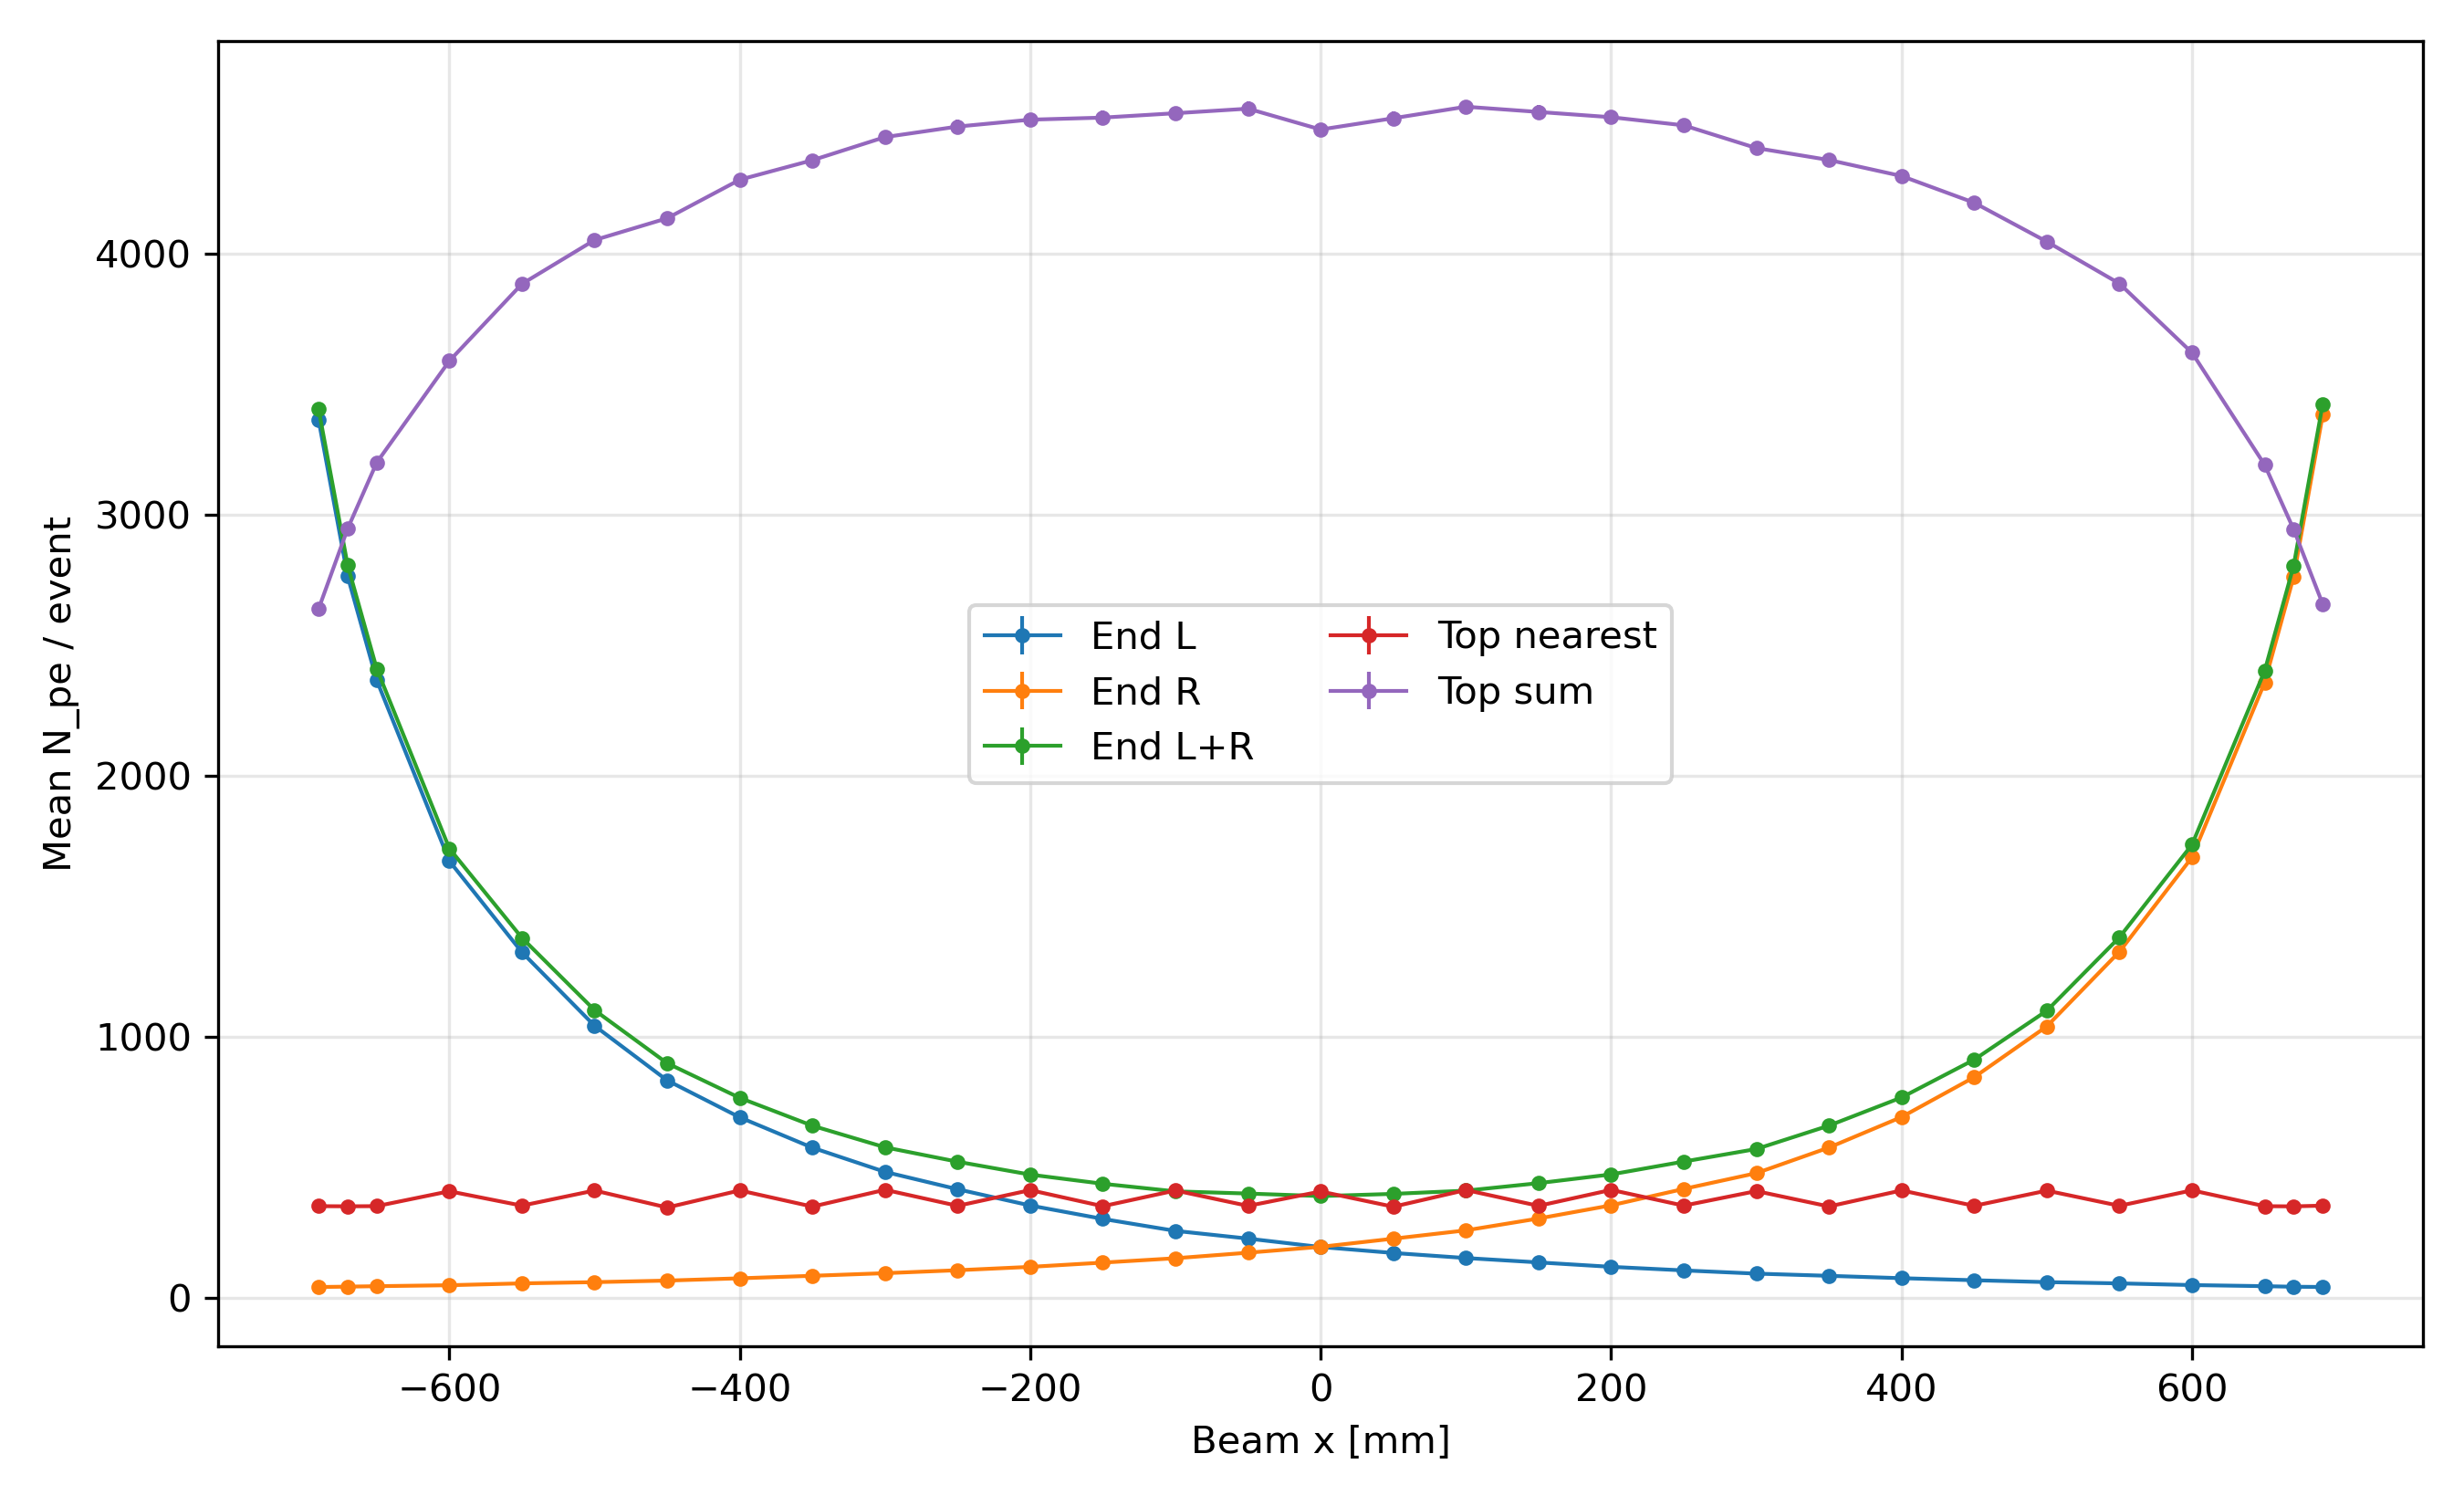
\includegraphics[width=\textwidth,height=0.78\textheight,keepaspectratio]{figs/P1_npe_vs_x.png}
\end{frame}
\begin{frame}{Top localization: full coverage diagonal}
\centering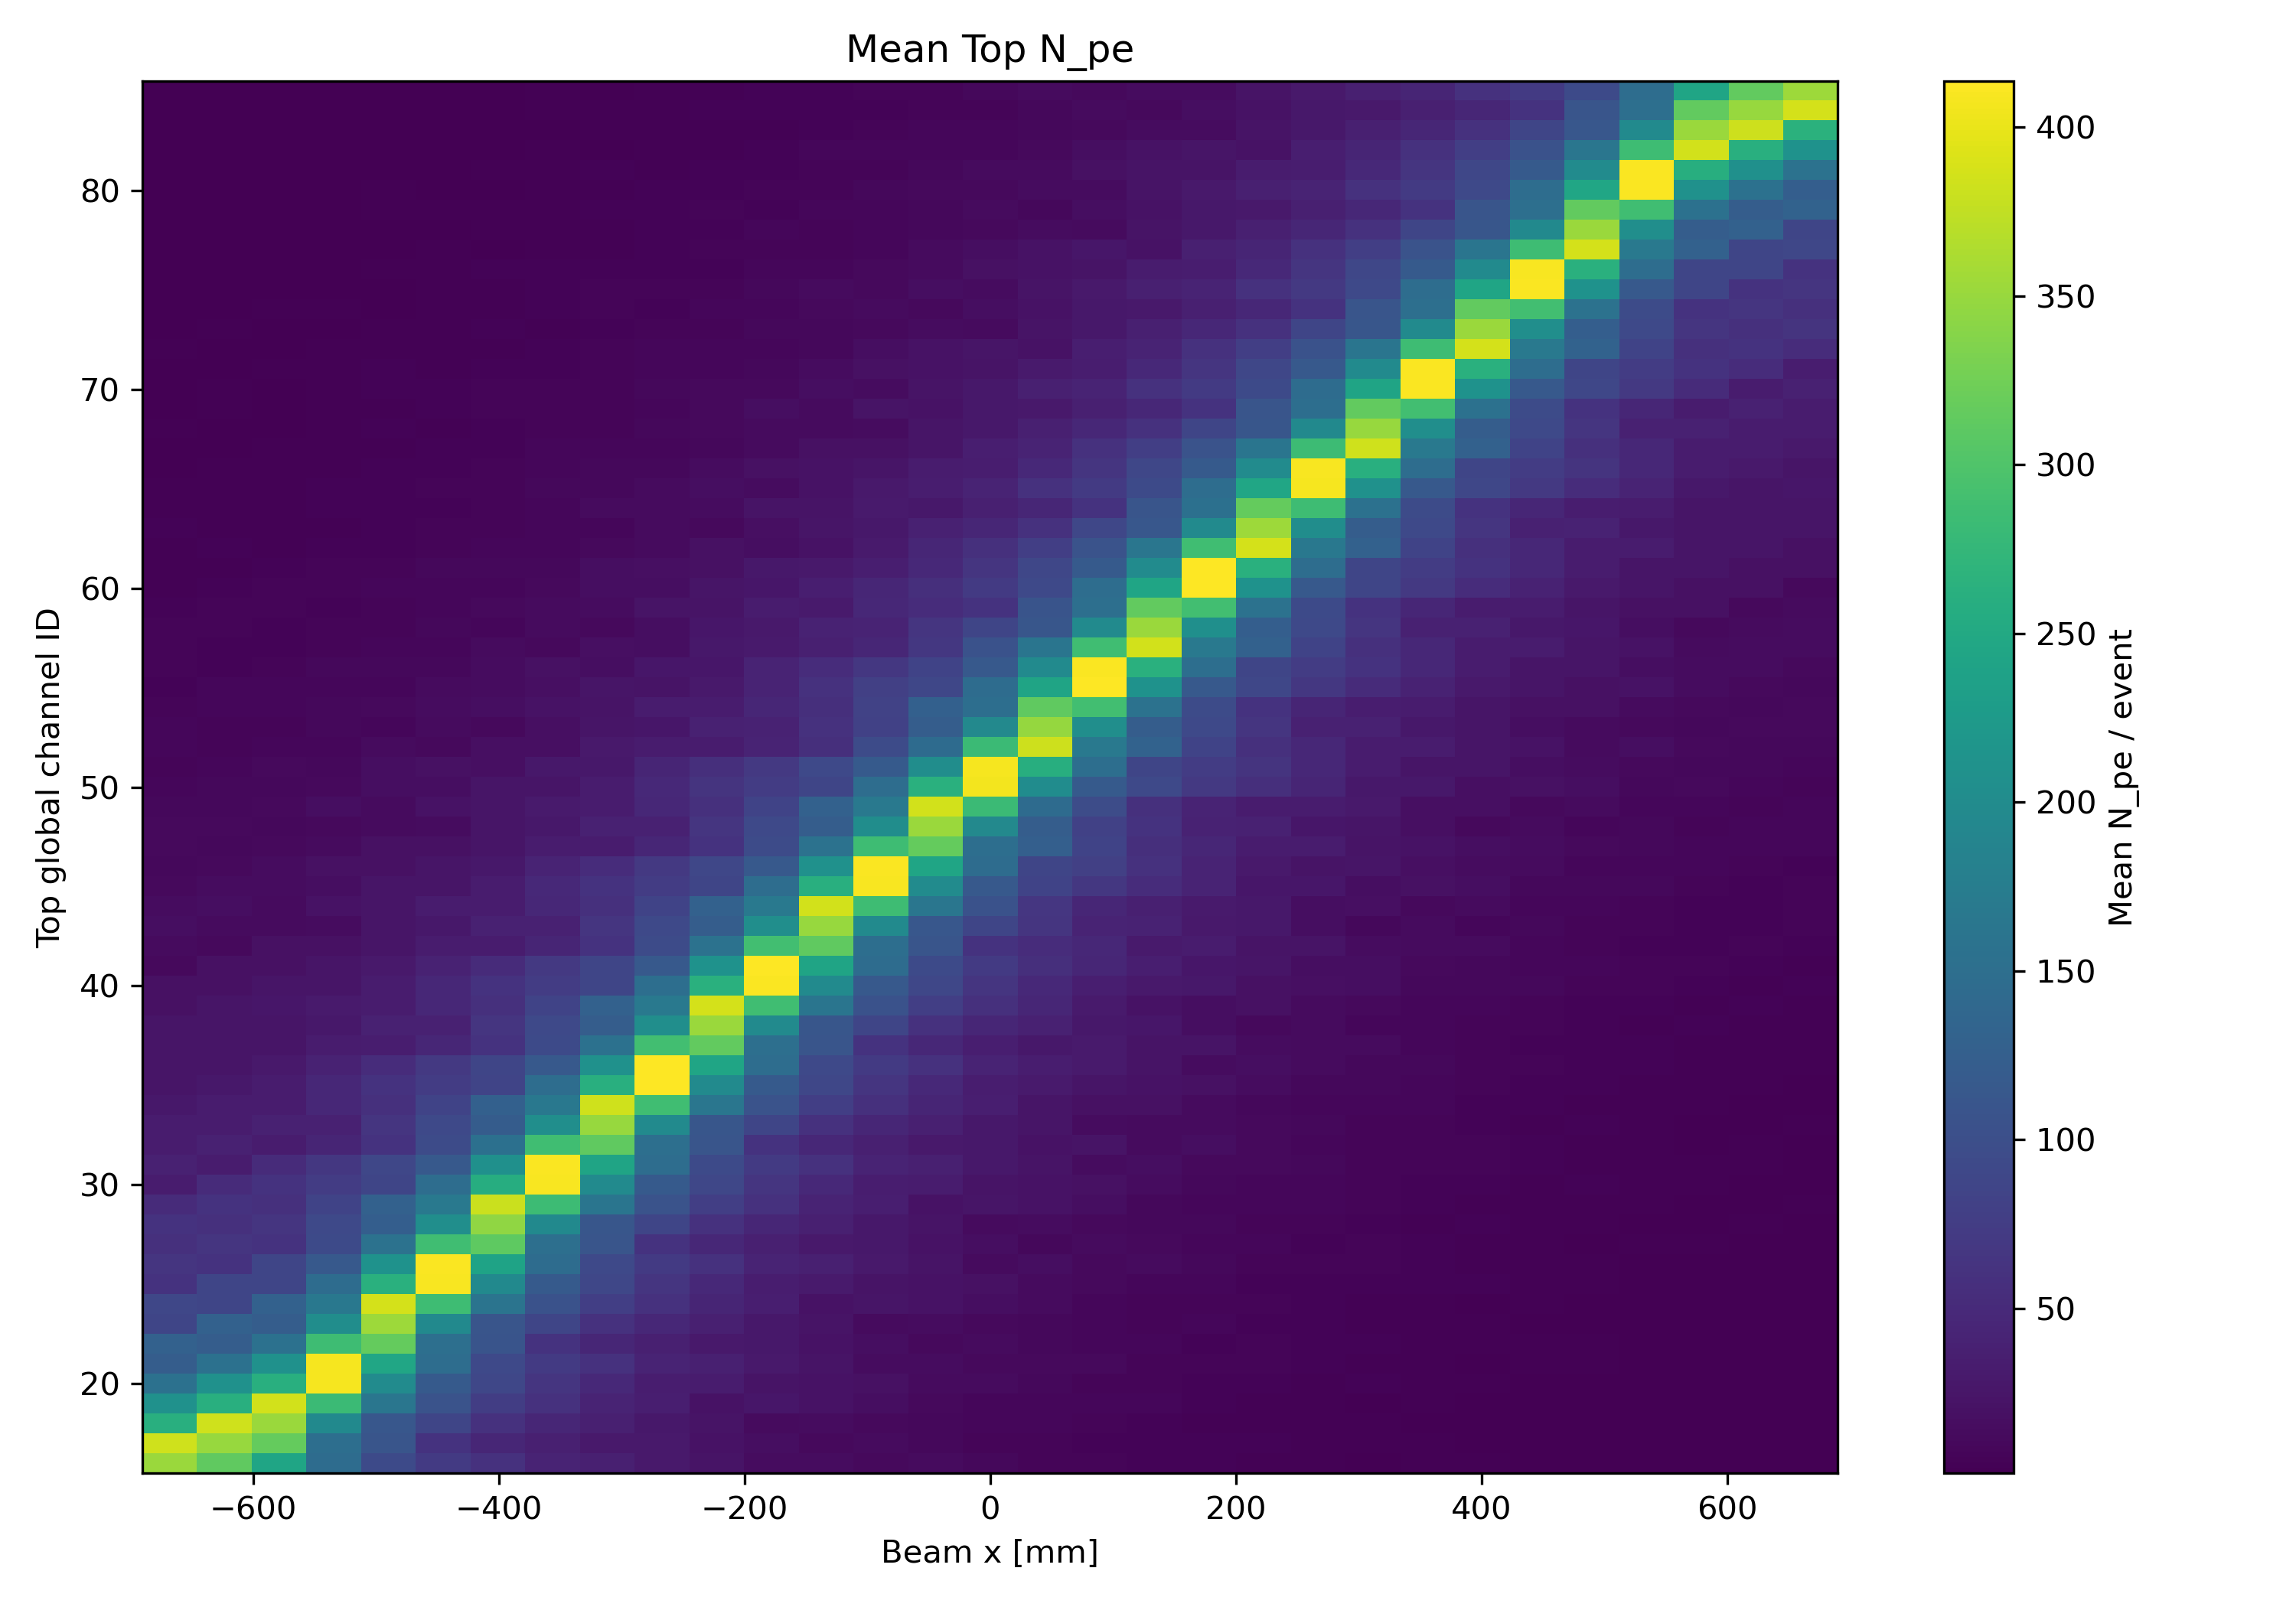
\includegraphics[width=\textwidth,height=0.78\textheight,keepaspectratio]{figs/P2_npe_heatmap_top.png}
\end{frame}
\begin{frame}{Attenuation and the historical mean-time slope}
\centering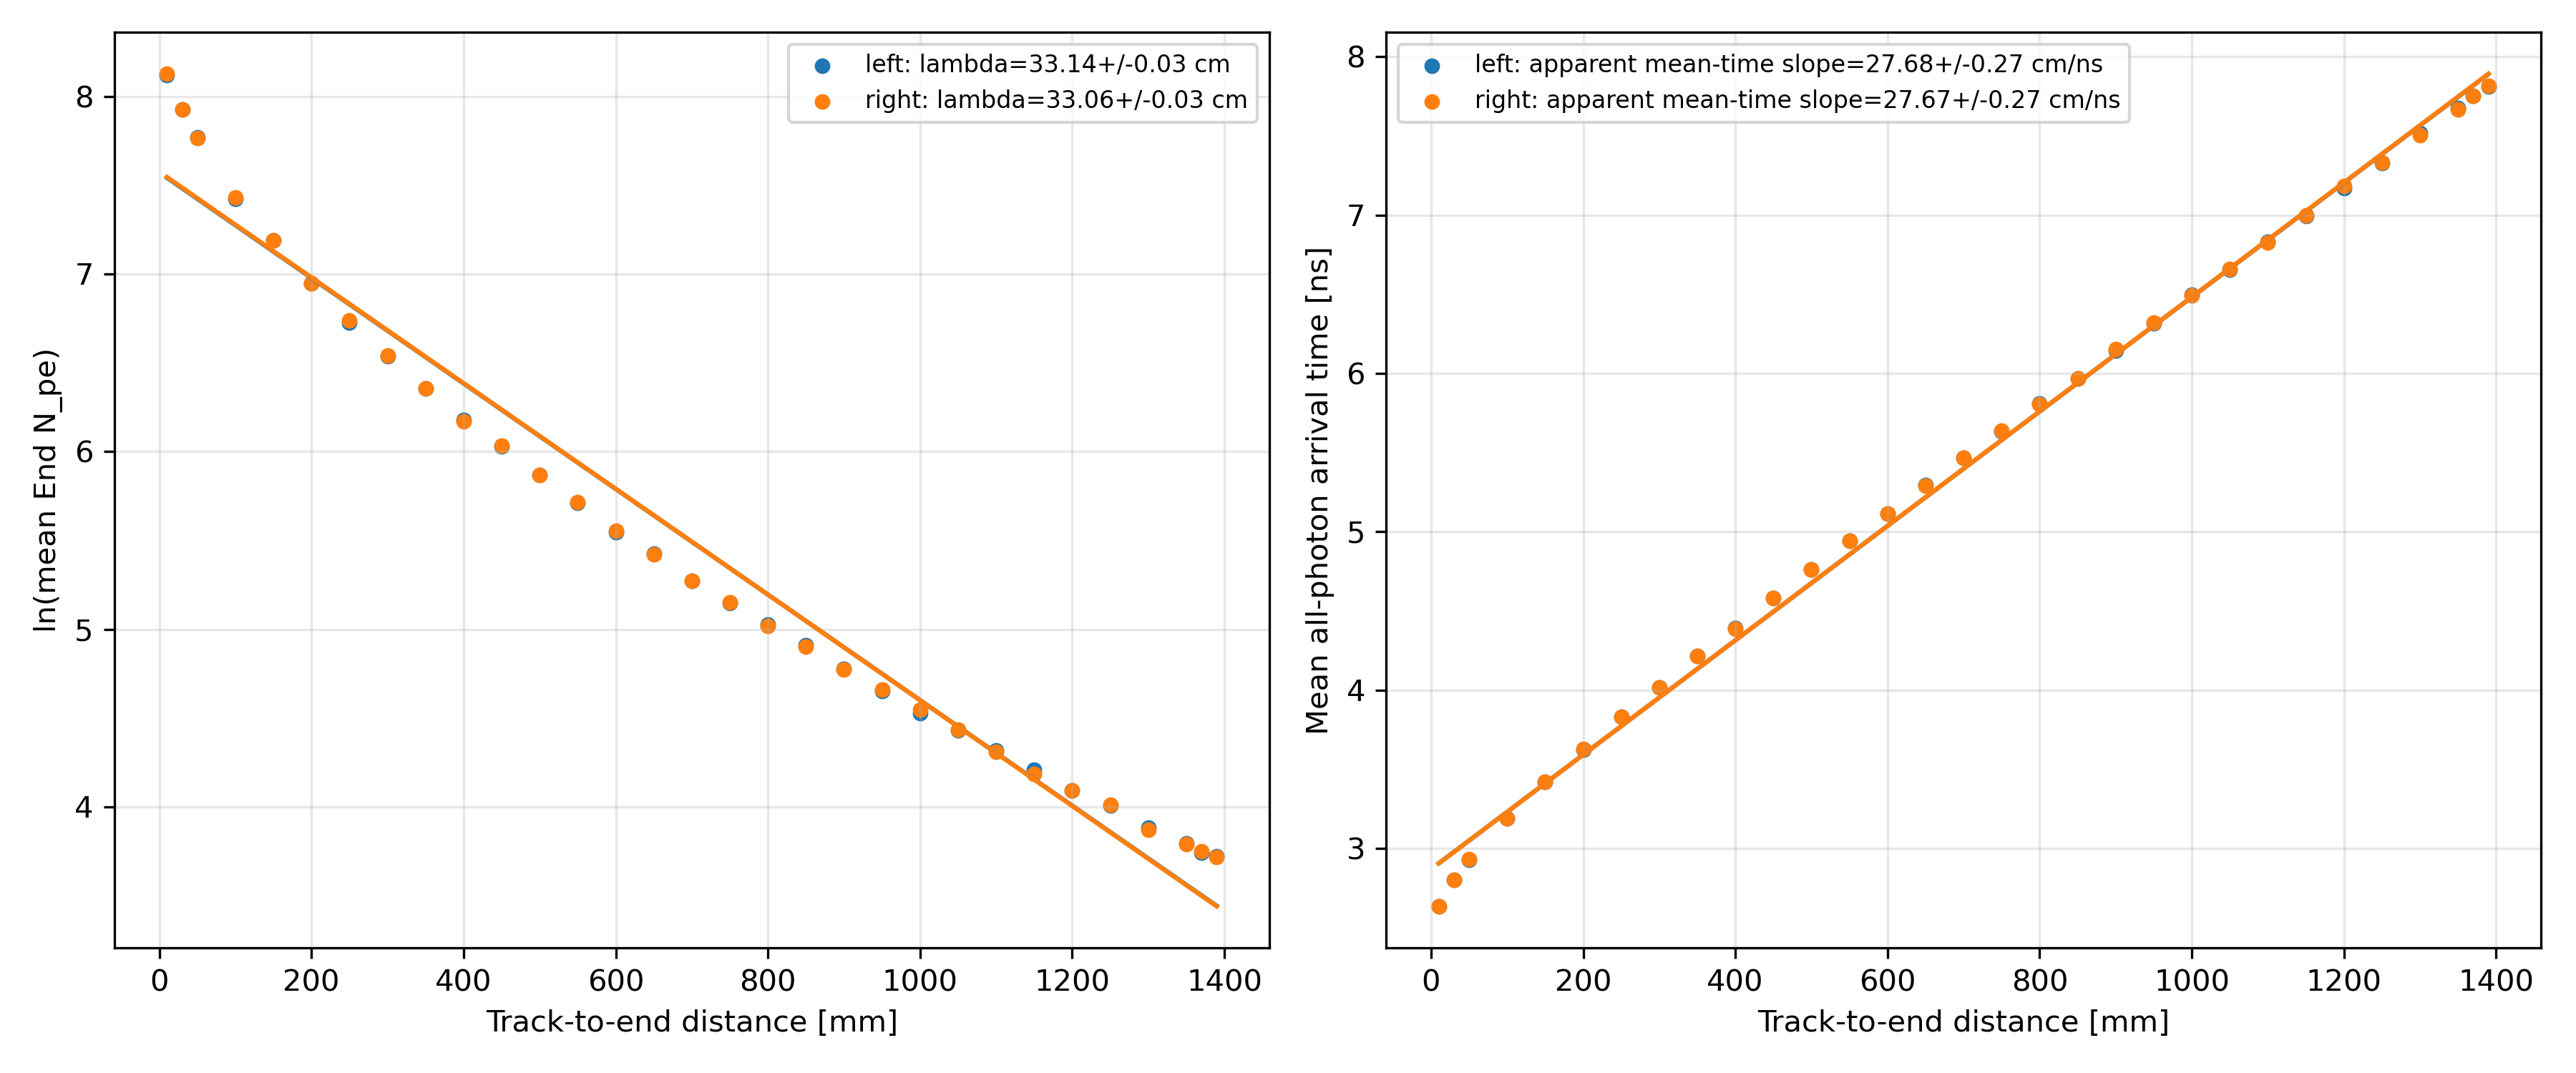
\includegraphics[width=\textwidth,height=0.78\textheight,keepaspectratio]{figs/fits_attenuation_velocity.png}\par\scriptsize $\lambda_{eff,L}=33.14\pm0.03$ cm, $\lambda_{eff,R}=33.06\pm0.03$ cm; the mean-time slope is tail-biased and is not a propagation velocity.
\end{frame}
\begin{frame}{Landau dominance: Fano factor versus mean Npe}
\centering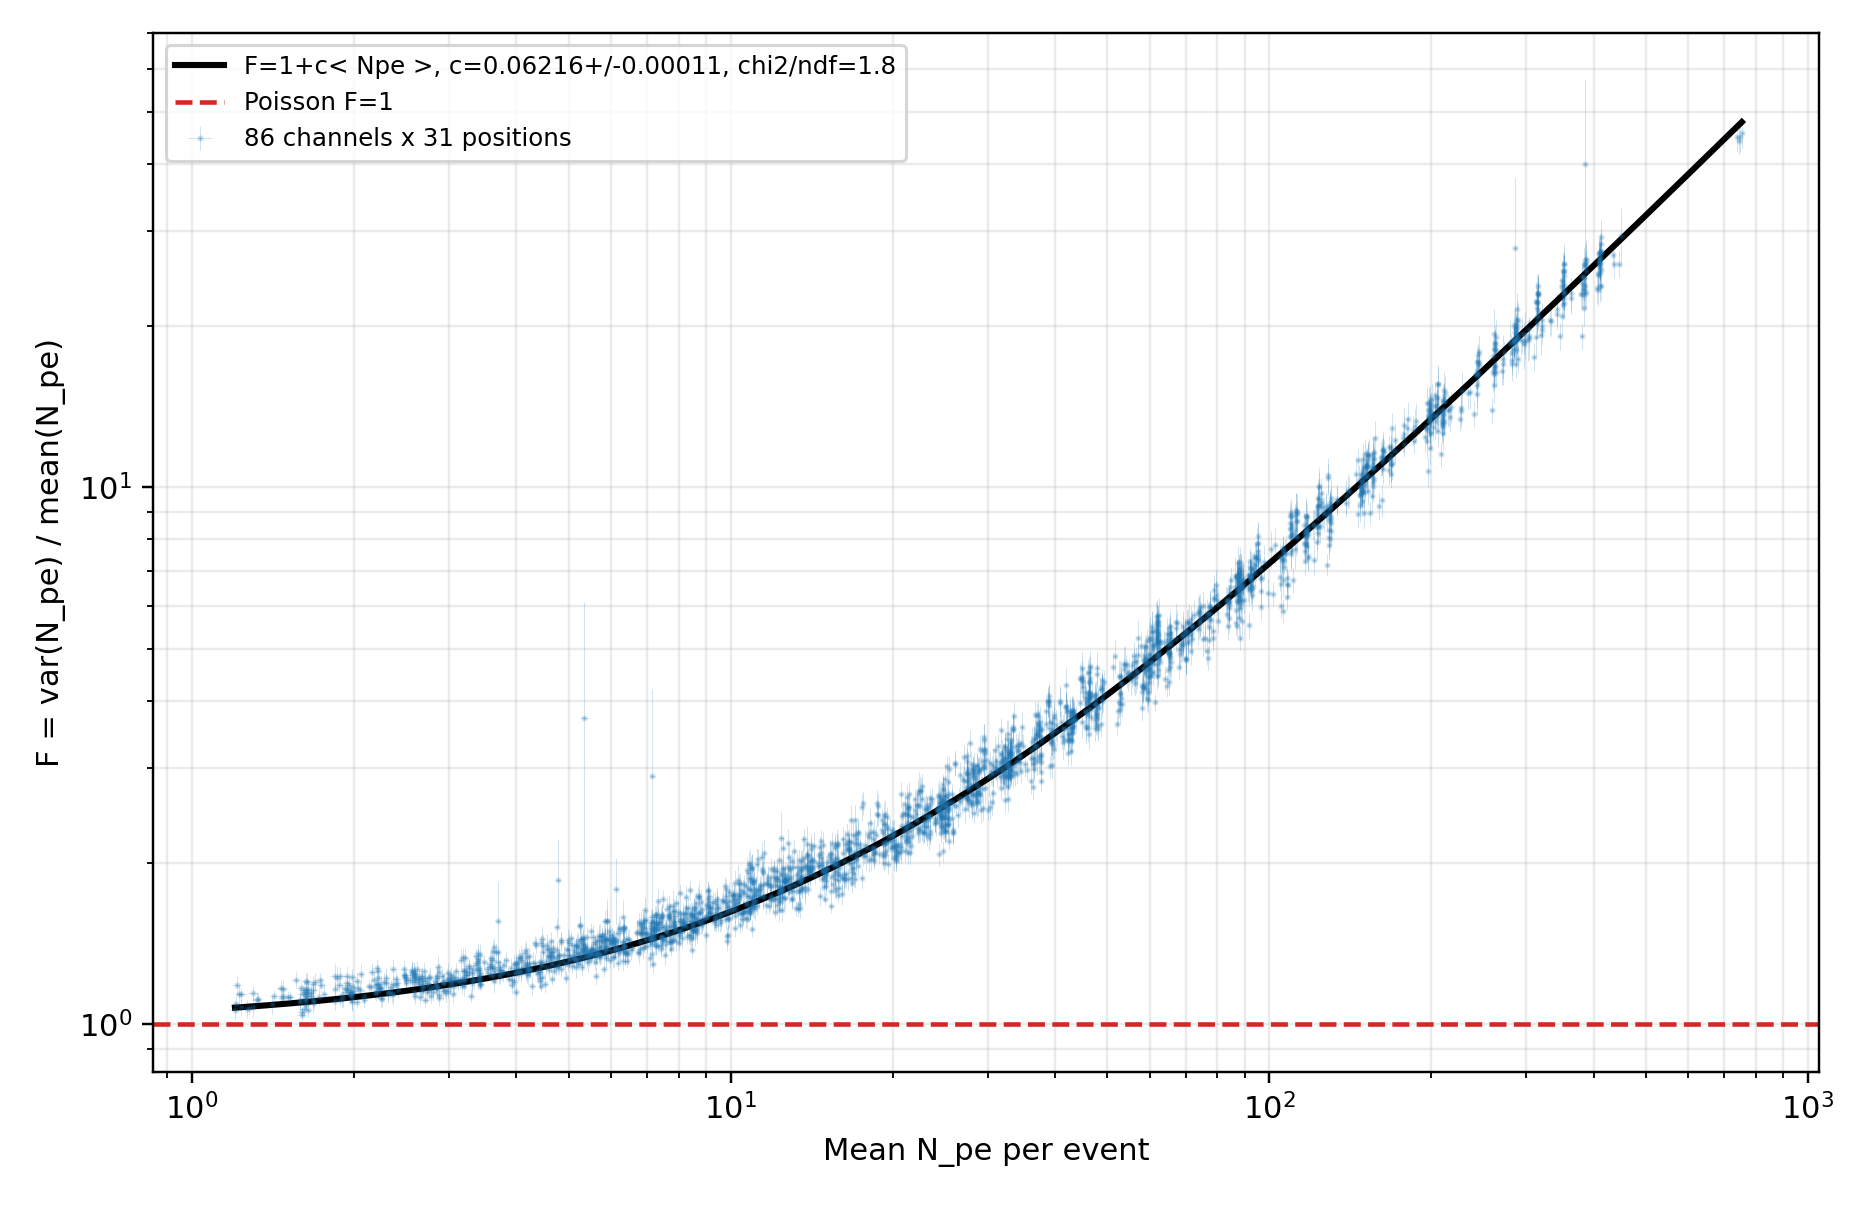
\includegraphics[width=\textwidth,height=0.78\textheight,keepaspectratio]{figs/exec10_fano_vs_mean.png}\par\scriptsize $F=1+c\langle N_{pe}\rangle$, $c=0.062162\pm0.000107$, $\chi^2/ndf=1.76$. Poisson $F=1$ is approached only at low light.
\end{frame}
\begin{frame}{High-light example: Moyal-Gaussian Landau proxy}
\centering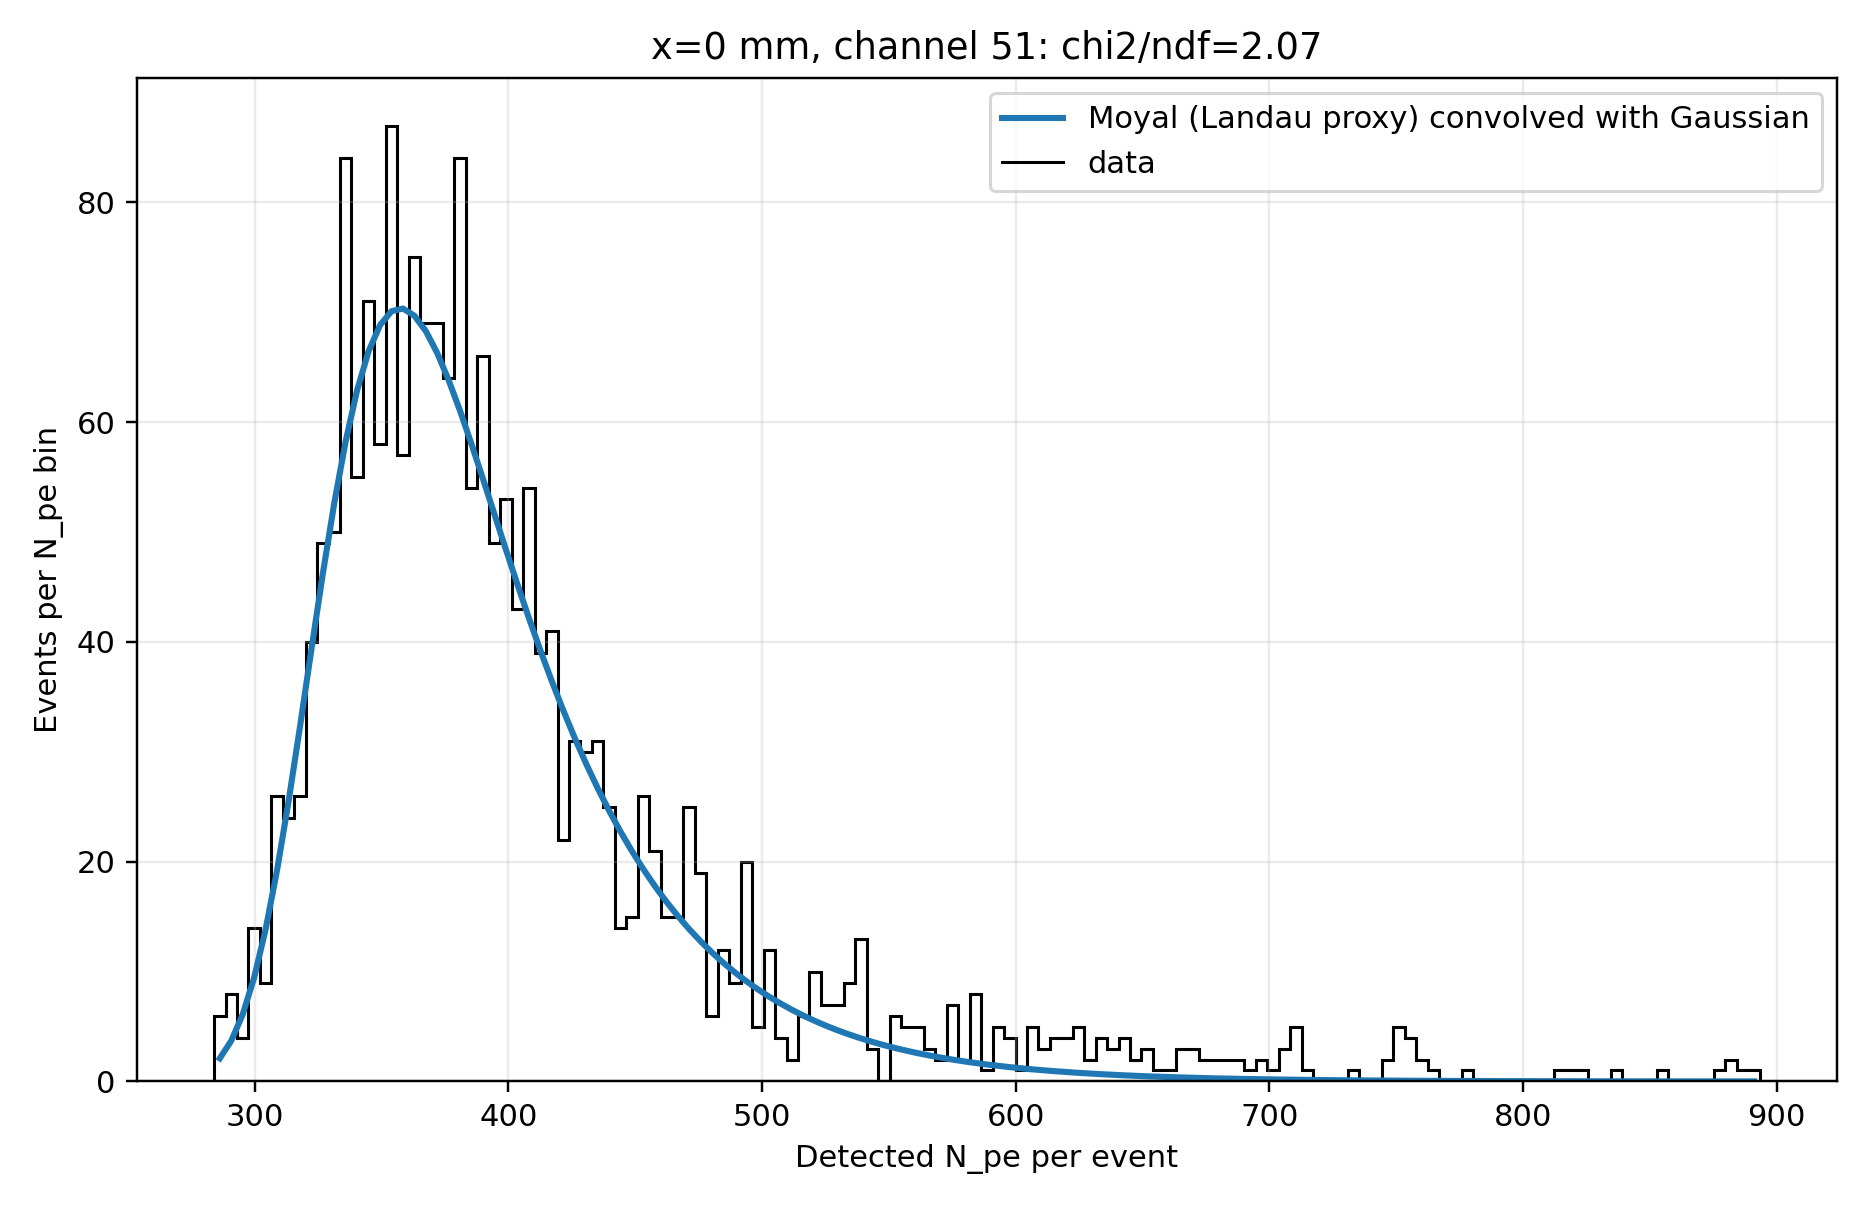
\includegraphics[width=\textwidth,height=0.78\textheight,keepaspectratio]{figs/exec10_landau_fit_example.png}\par\scriptsize Moyal approximates Landau. Some channels have poor chi2 or an unidentifiable Gaussian width; all are recorded in \texttt{exec10\_landau\_mpv.csv}.
\end{frame}
\begin{frame}{Arrival-time examples: absolute rate and normalized shape}
\centering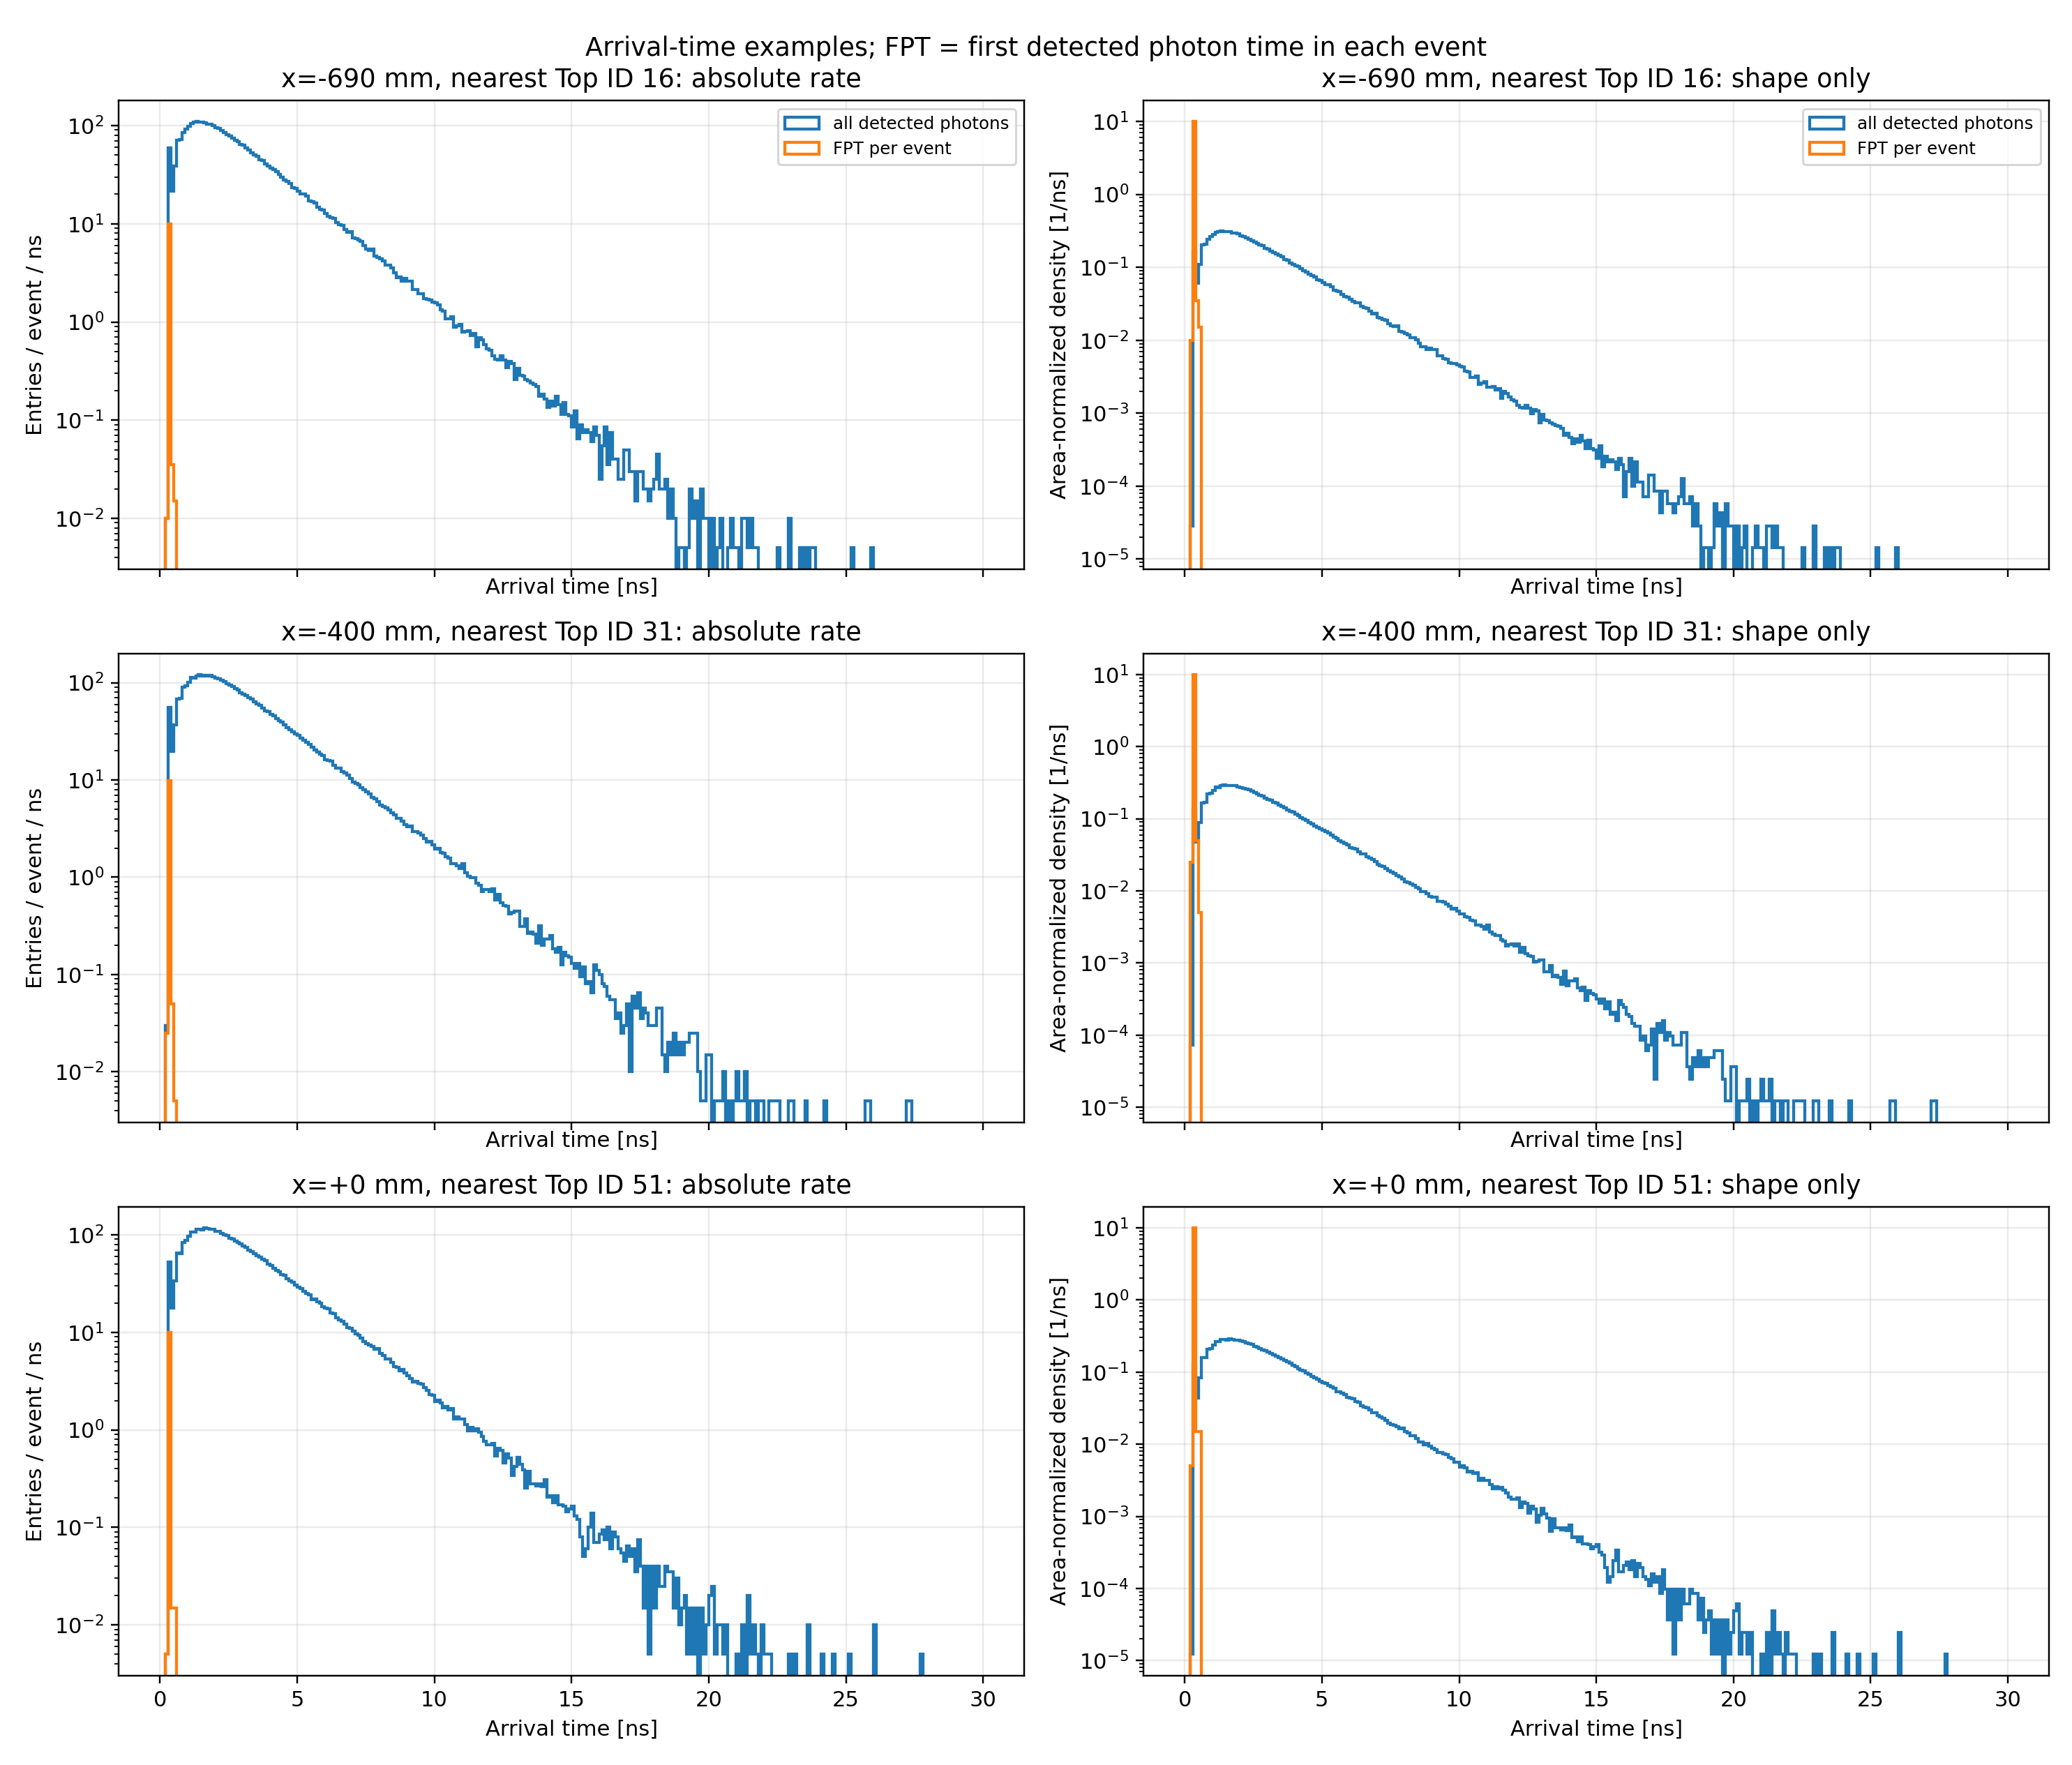
\includegraphics[width=\textwidth,height=0.78\textheight,keepaspectratio]{figs/P5_tdist_examples.png}\par\scriptsize Left: entries per event per ns. Right: the same distributions normalized to area 1. FPT is the first detected photon time in each event.
\end{frame}
\begin{frame}{Mean arrival time and FPT versus x}
\centering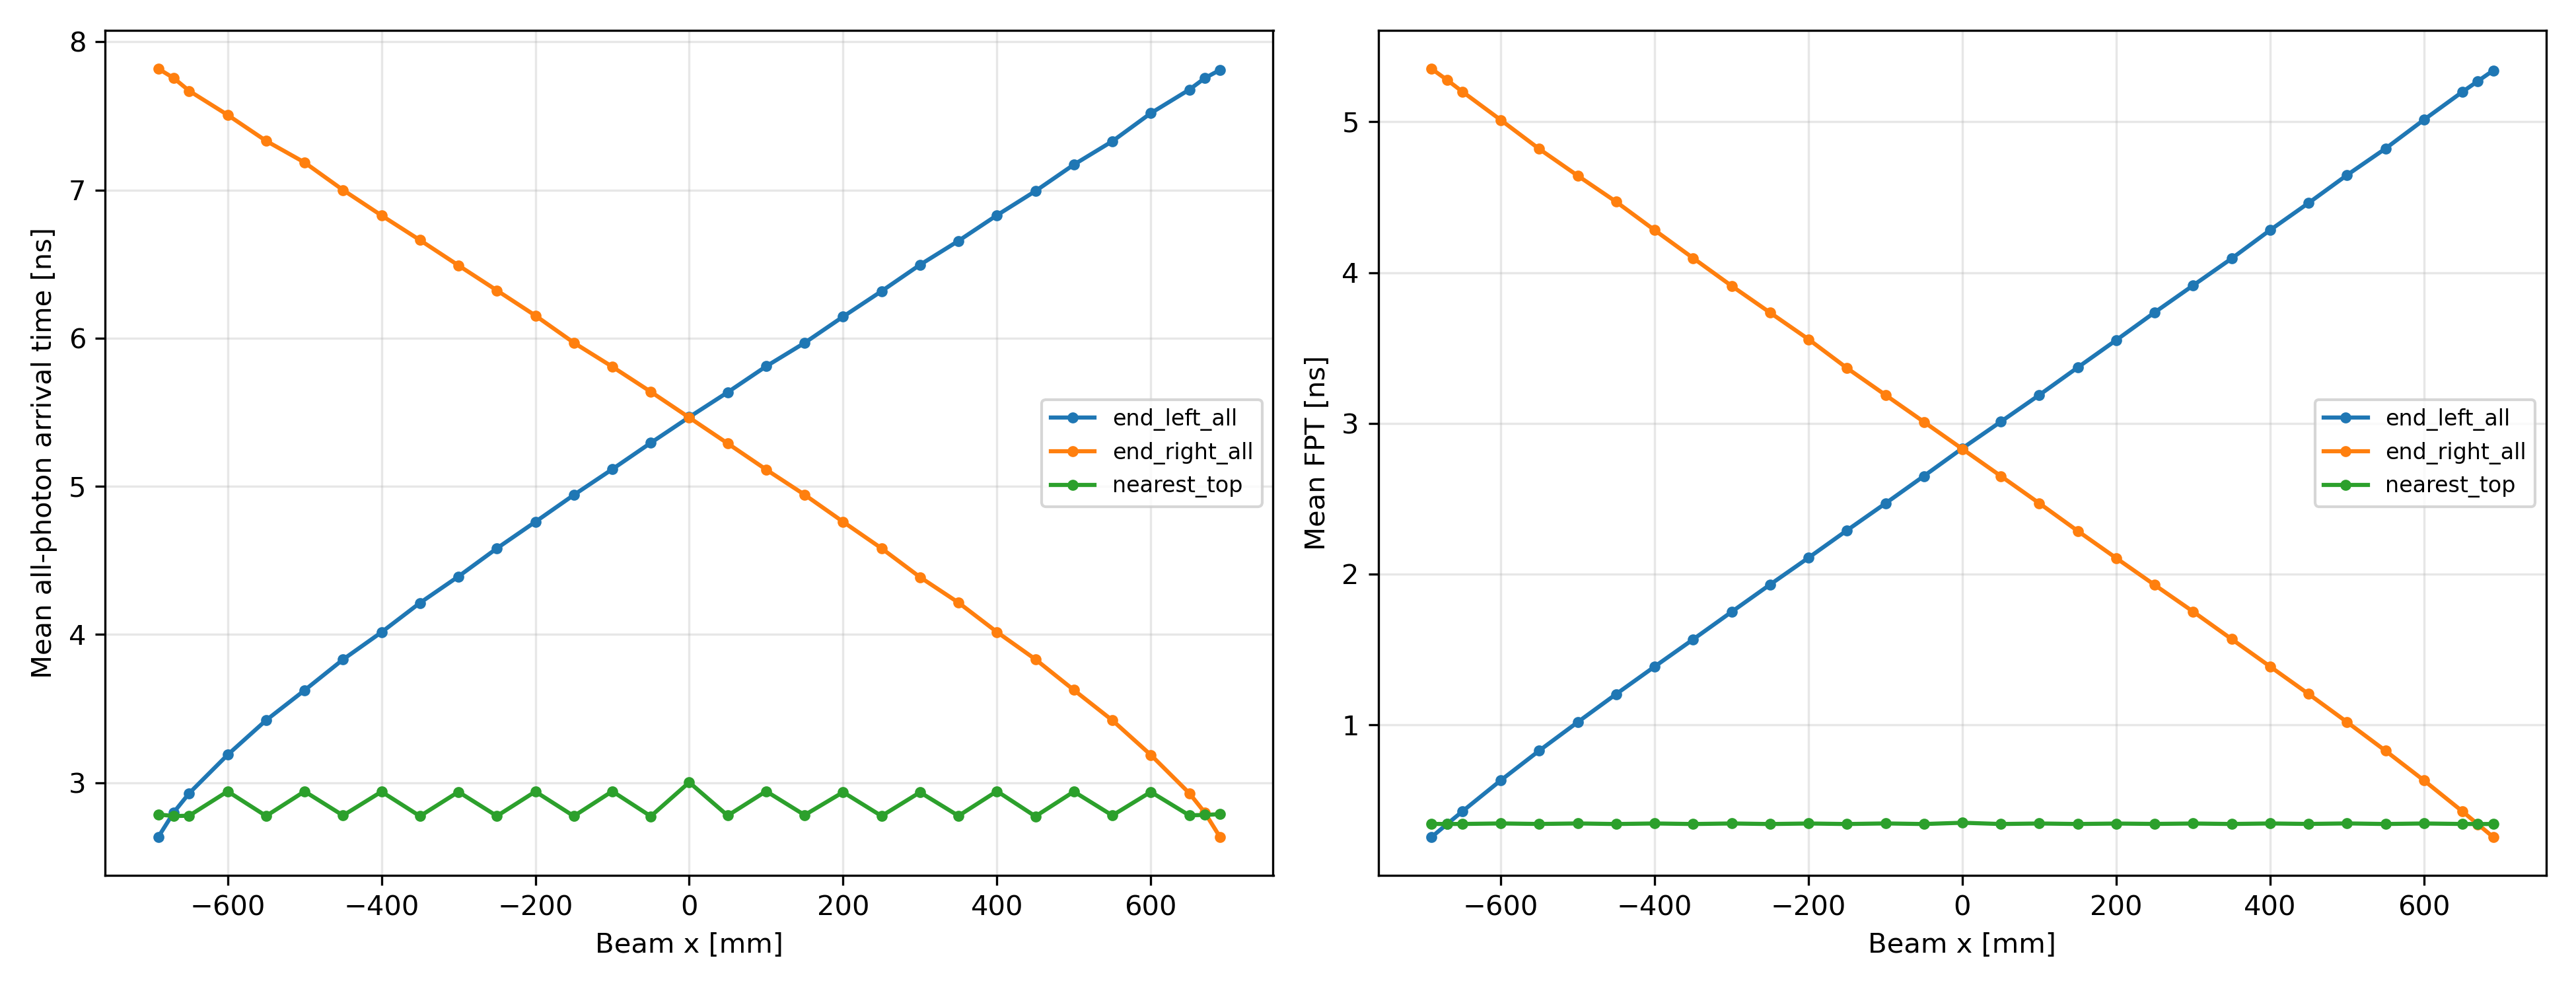
\includegraphics[width=\textwidth,height=0.78\textheight,keepaspectratio]{figs/P6_tmean_vs_x.png}
\end{frame}
\section{Window effect and timing}
\begin{frame}{Nearest-Top Landau/Moyal MPVs at key positions}

\centering\small
\begin{tabular}{rrrrr}\toprule
$x$ [mm] & channel & MPV [Npe] & Landau width [Npe] & $\chi^2/ndf$ \\ \midrule
-690 & 16 & $304.4\pm1.0$ & $26.9\pm0.9$ & 1.76 \\
-650 & 18 & $302.4\pm1.0$ & $26.3\pm0.9$ & 1.04 \\
-400 & 31 & $356.9\pm1.1$ & $29.3\pm1.0$ & 1.33 \\
+0 & 51 & $355.4\pm1.1$ & $26.7\pm0.9$ & 2.07 \\
+400 & 70 & $356.4\pm1.2$ & $29.1\pm1.0$ & 1.51 \\
+650 & 83 & $304.1\pm1.0$ & $26.6\pm0.9$ & 1.61 \\
+690 & 85 & $304.7\pm1.0$ & $25.6\pm0.9$ & 1.31 \\
\bottomrule\end{tabular}
\begin{block}{Interpretation}
The right tail originates primarily from Landau-like energy-loss fluctuations; Poisson
counting dominates only in the few-PE limit. MPVs are future inputs for the pending
test-beam ToT(NPE) calibration comparison.
\end{block}

\end{frame}
\begin{frame}{Window-track collection effect: five-run test}

\begin{columns}[T]\column{0.47\textwidth}
\scriptsize\resizebox{\textwidth}{!}{\begin{tabular}{lrr}\toprule
Run & contrast [Npe] & significance \\ \midrule
Existing -650 & $34.60\pm2.94$ & $11.78$ \\
A -652 center & $2.86\pm2.65$ & $1.08$ \\
B -642 midpoint & $-0.33\pm3.35$ & $-0.10$ \\
C1 -648 (+4 mm) & $21.08\pm3.20$ & $6.59$ \\
C2 -654 mirror & $34.38\pm2.95$ & $11.64$ \\
\bottomrule\end{tabular}}
\column{0.51\textwidth}
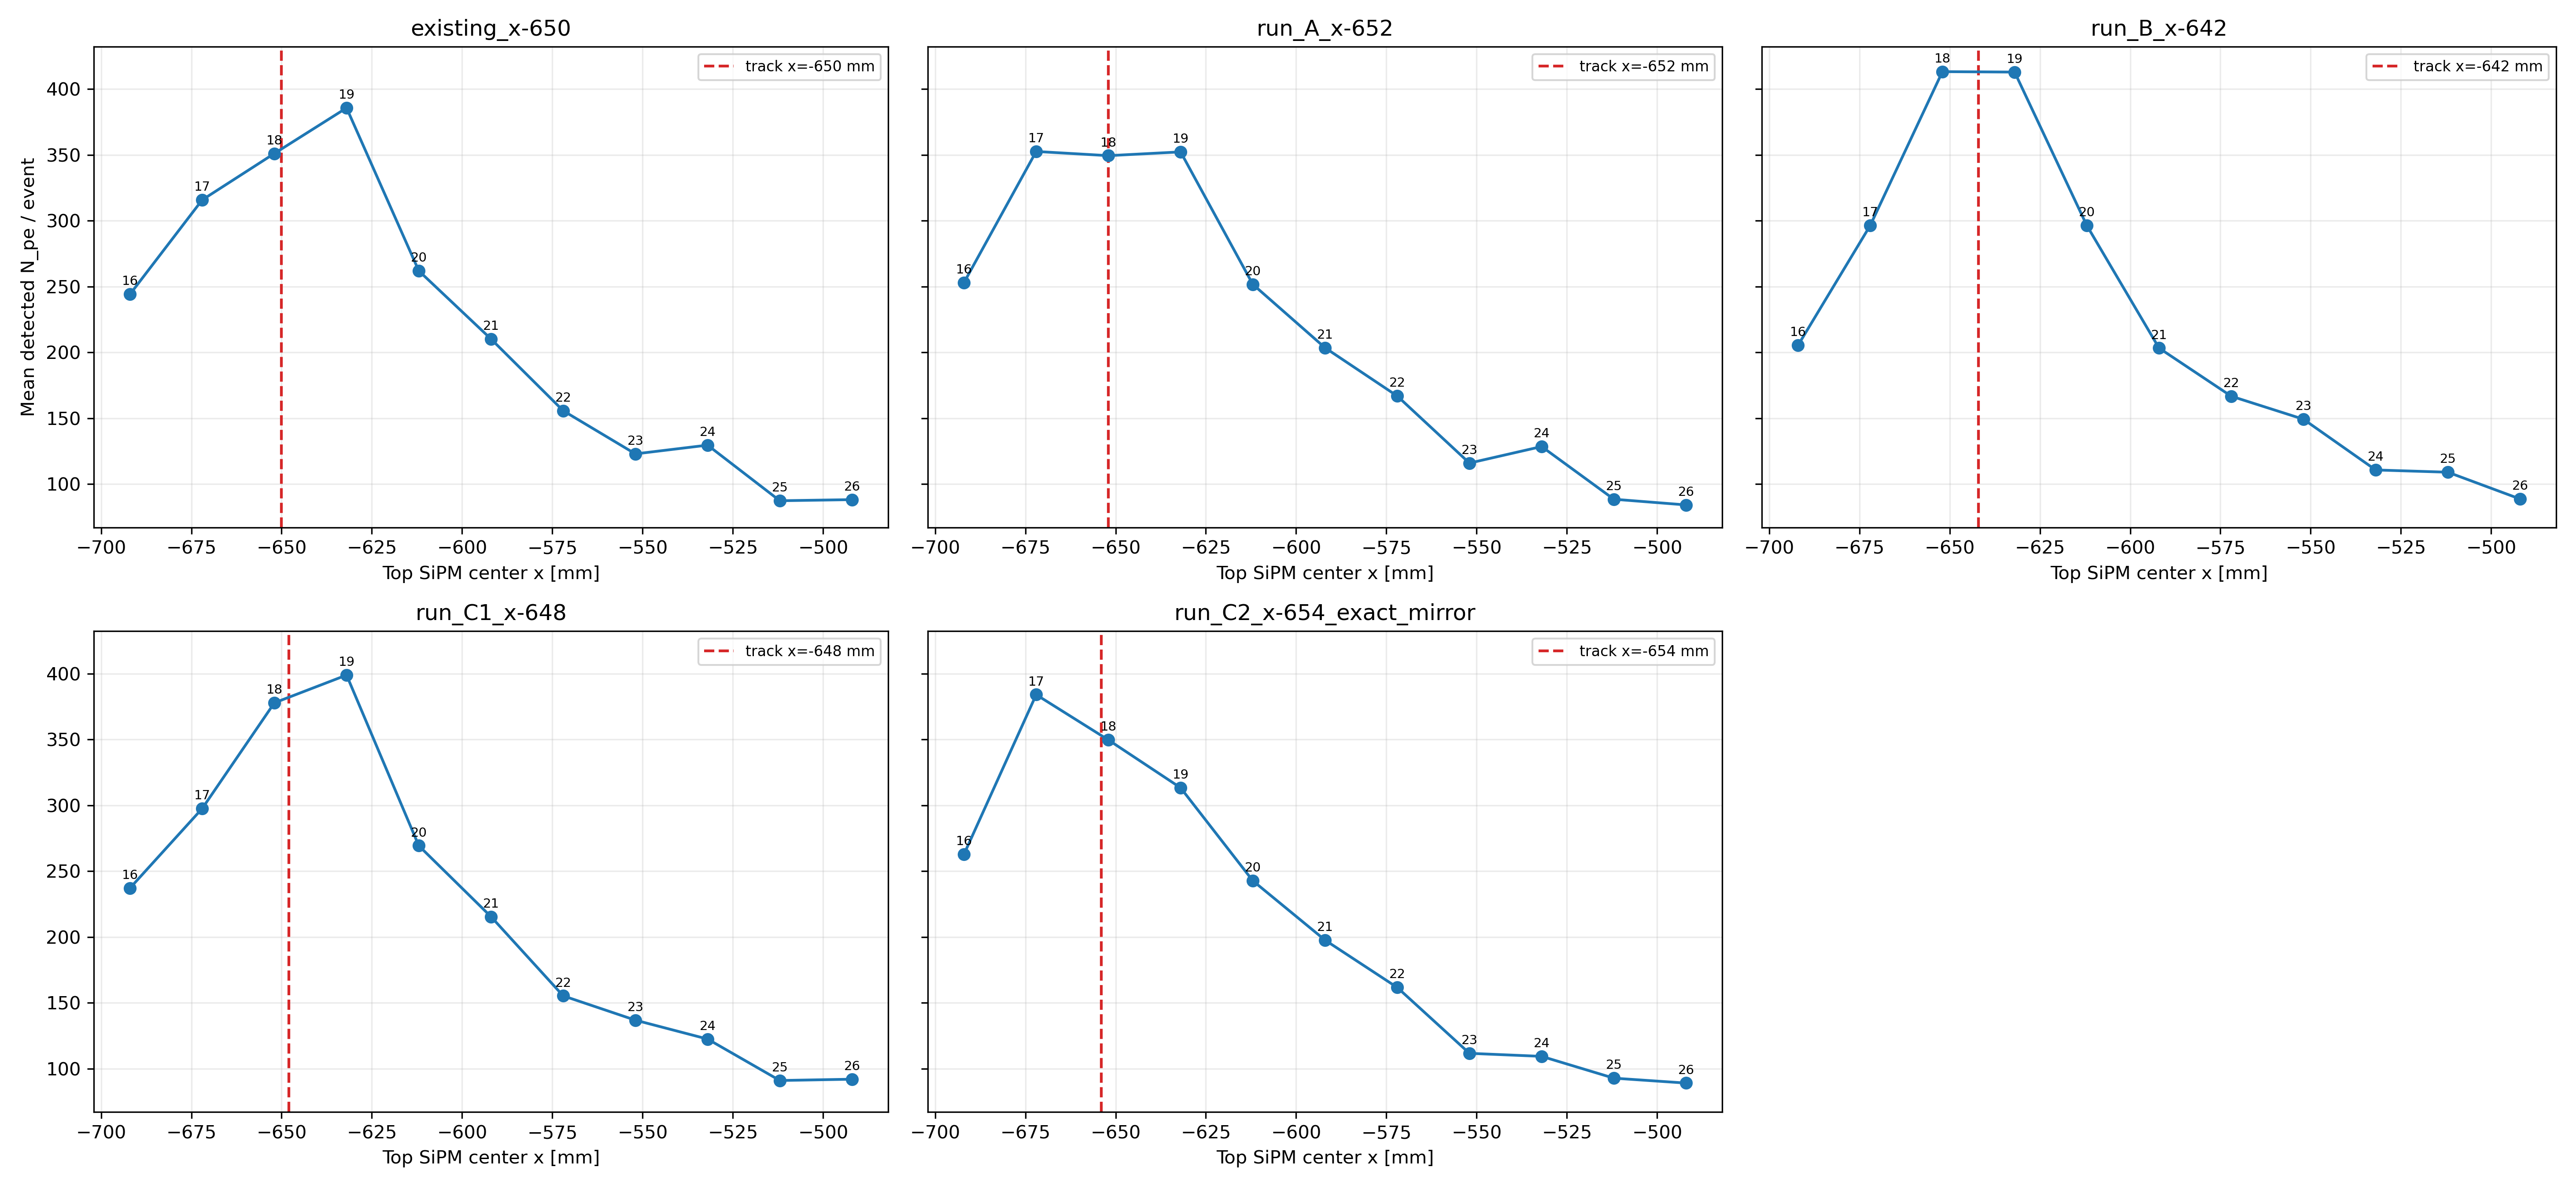
\includegraphics[width=\textwidth]{figs/exec08b_window_dip_profiles.png}
\end{columns}
\begin{block}{Finding}
Local symmetric $\pm2$ mm effect: about 9.8\% at about 12 sigma; null when centered
and at midpoint. The scan and channel map remain valid.
\end{block}

\end{frame}
\begin{frame}{Intrinsic End SUM4 timing}
\centering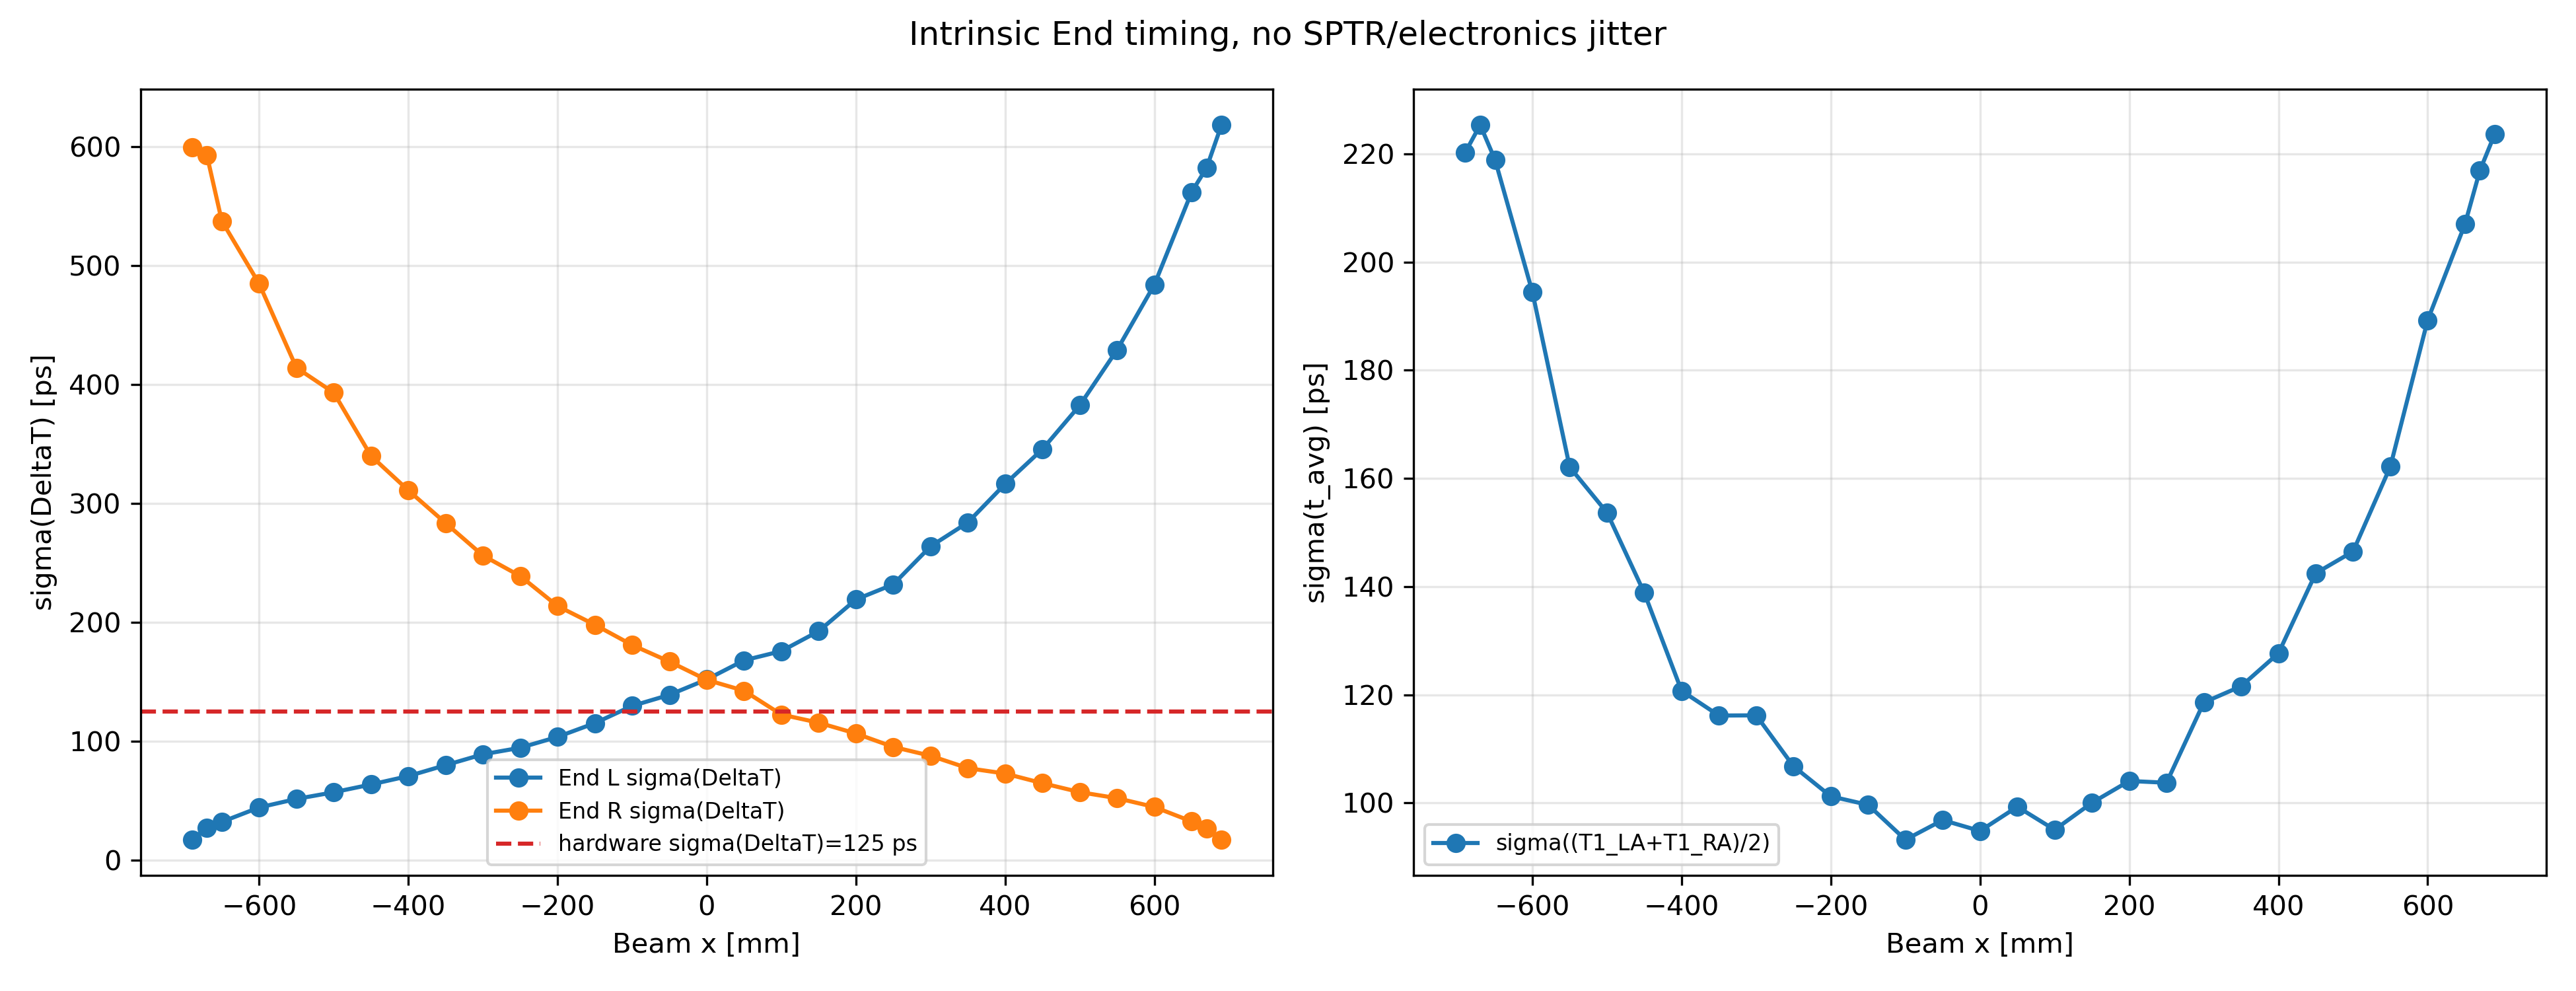
\includegraphics[width=\textwidth,height=0.78\textheight,keepaspectratio]{figs/P7_deltaT_end.png}\par\scriptsize $\sigma_{group}=\sigma(\Delta T_{AB})/\sqrt{2}$; no SPTR/jitter. The 88 ps hardware context is not directly comparable.
\end{frame}
\begin{frame}{Timing gate lifted: narrower EndTop is physical}

\begin{columns}[T]\column{0.48\textwidth}
\scriptsize\resizebox{\textwidth}{!}{\begin{tabular}{rrrrr}\toprule
$x$ & side & EndTop [ps] & End-only [ps] & ratio \\ \midrule
-400 & L & $50.0\pm0.8$ & $66.1\pm0.5$ & $0.756\pm0.013$ \\
-400 & R & $219.9\pm3.5$ & $248.4\pm1.8$ & $0.885\pm0.015$ \\
+0 & L & $107.5\pm1.7$ & $131.4\pm0.9$ & $0.818\pm0.014$ \\
+0 & R & $107.2\pm1.7$ & $129.5\pm0.9$ & $0.828\pm0.014$ \\
+400 & L & $223.8\pm3.5$ & $247.5\pm1.8$ & $0.904\pm0.016$ \\
+400 & R & $51.5\pm0.8$ & $65.9\pm0.5$ & $0.781\pm0.014$ \\
\bottomrule\end{tabular}}
\column{0.50\textwidth}
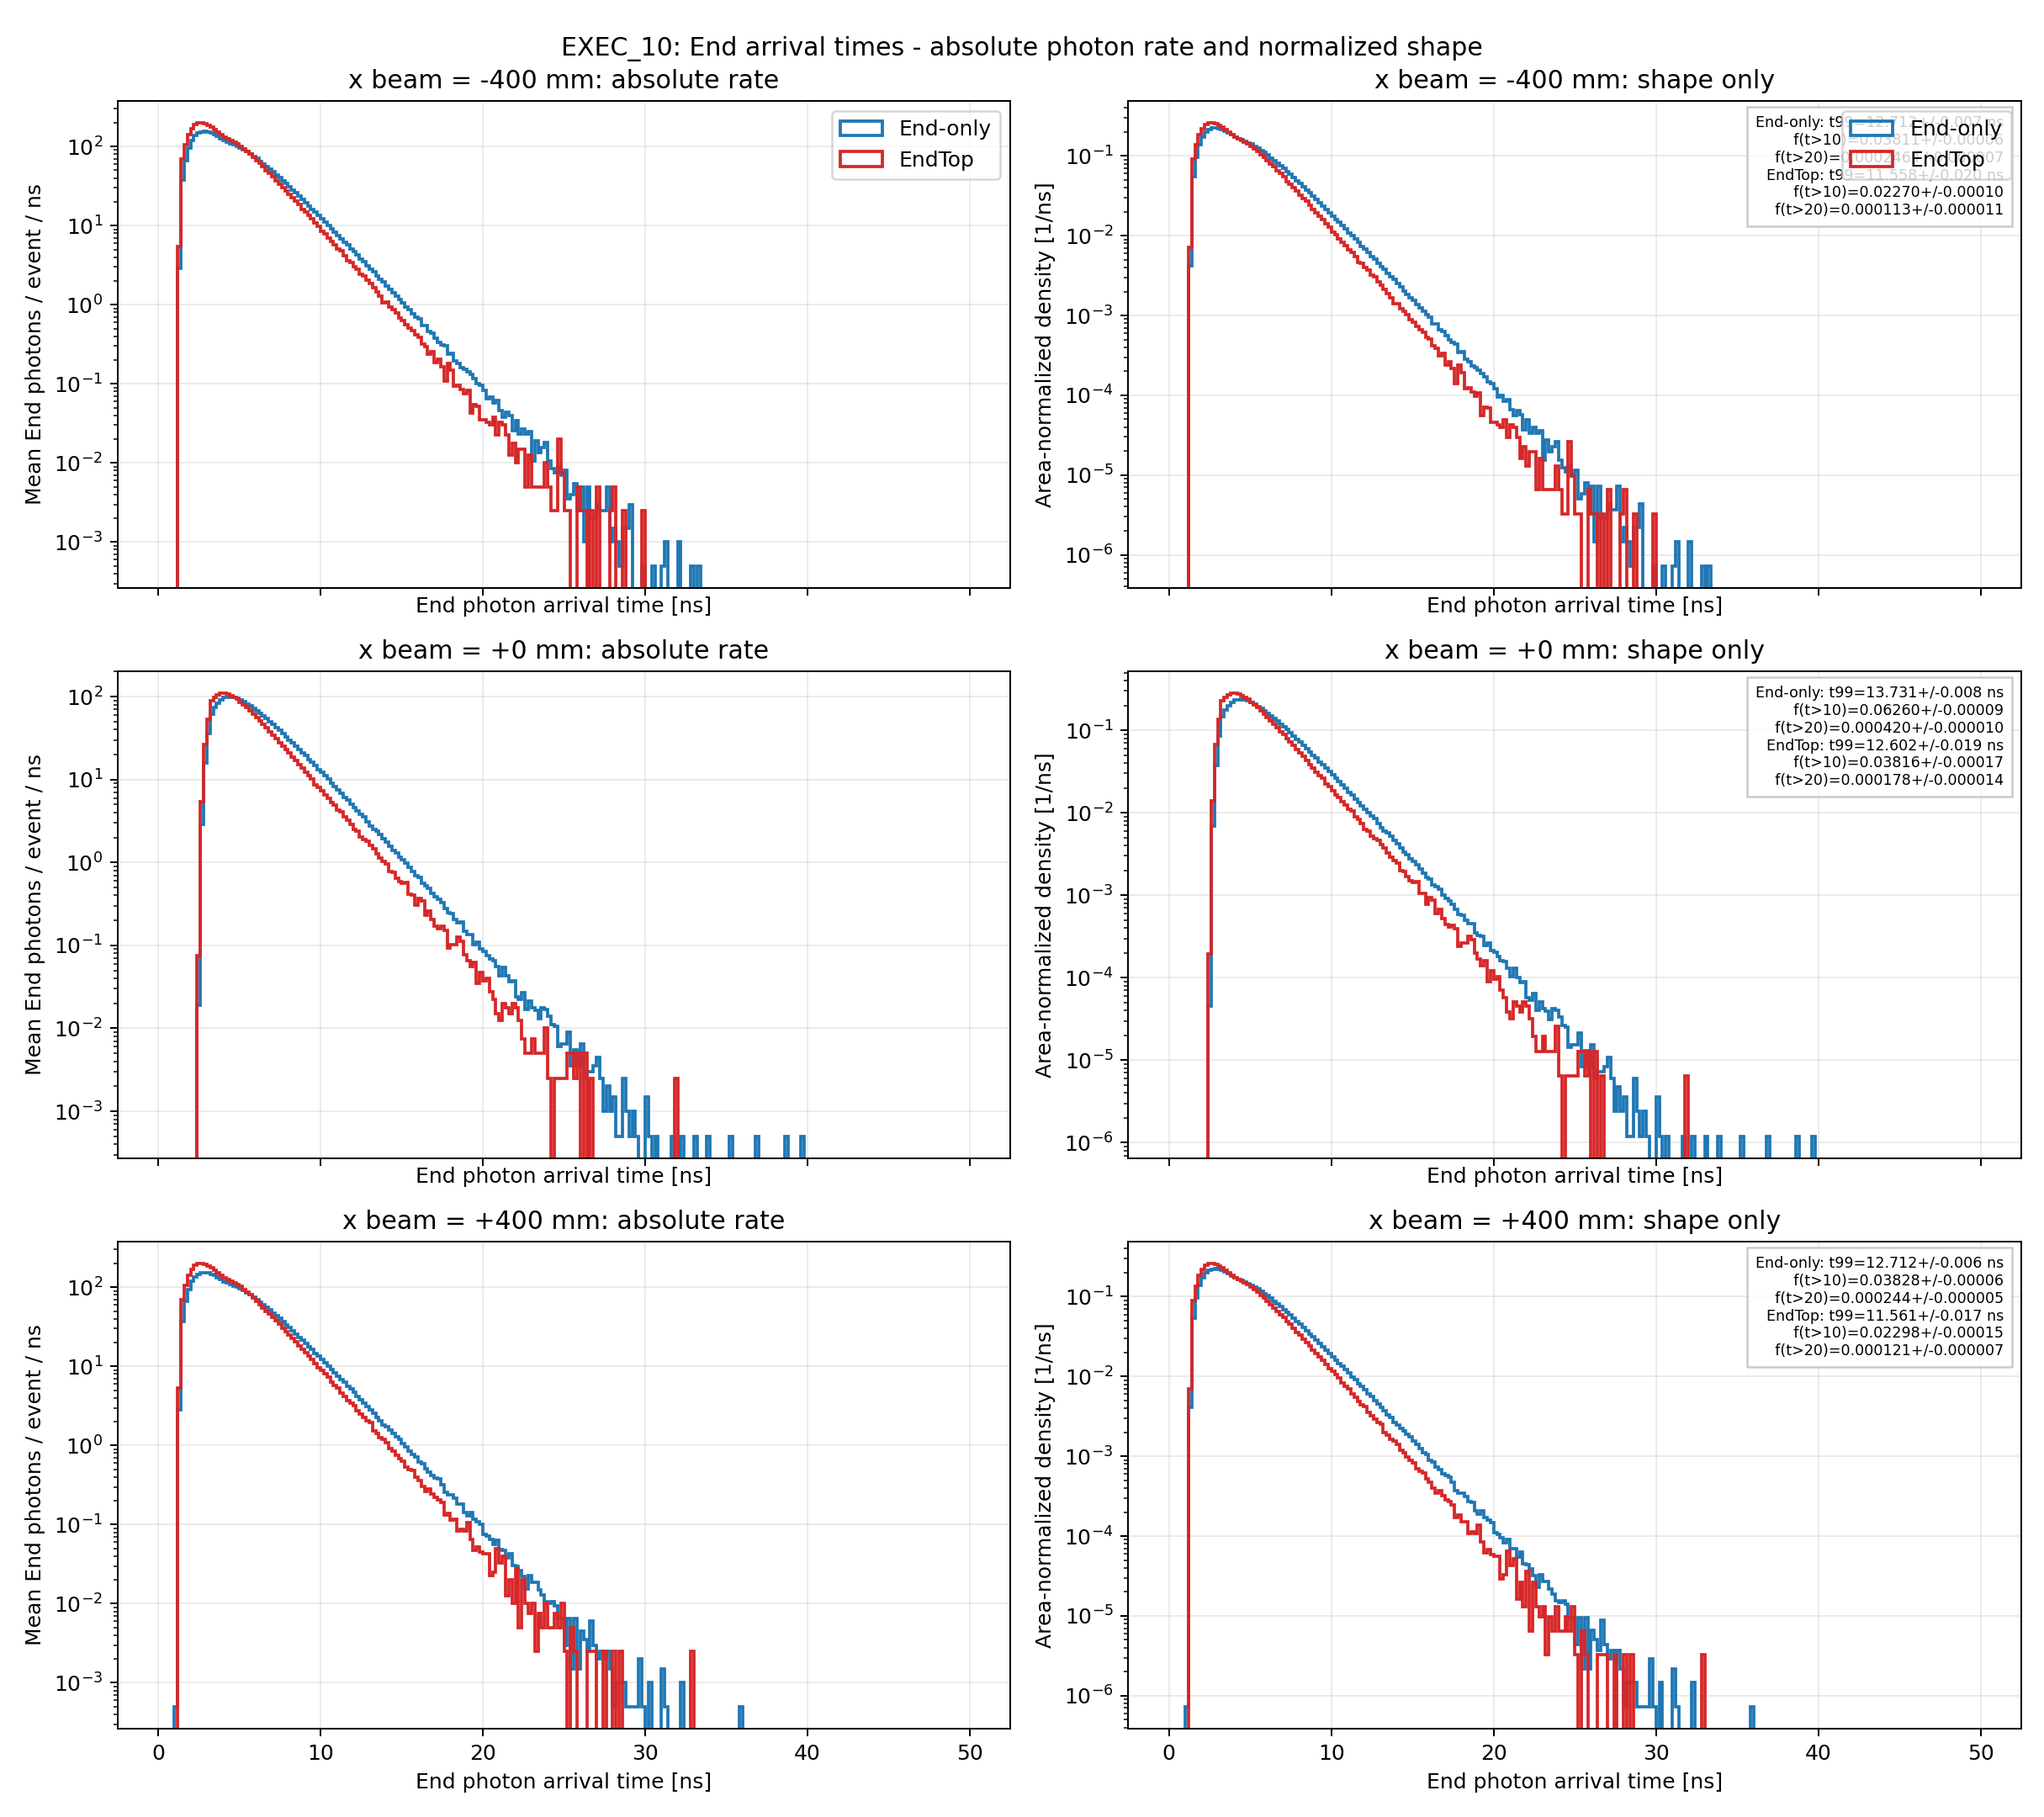
\includegraphics[width=0.88\textwidth]{figs/exec09_tail_comparison.png}
\end{columns}
\begin{alertblock}{Confirmed mechanism}
Across $x=0,\pm400$ mm, EndTop lowers $t99$ by
1.14 ns and suppresses late fractions
at more than 10.3 sigma.
\end{alertblock}
\tiny Left panels show absolute End photons/event/ns. Right panels normalize
each distribution to area 1 and isolate shape: the $t>10$ ns tail is suppressed in EndTop
because multiply reflected photons have more opportunities to meet a Top window.

\end{frame}
\begin{frame}{Apparent timing slopes: no propagation estimator passes}

\begin{columns}[T]\column{0.62\textwidth}
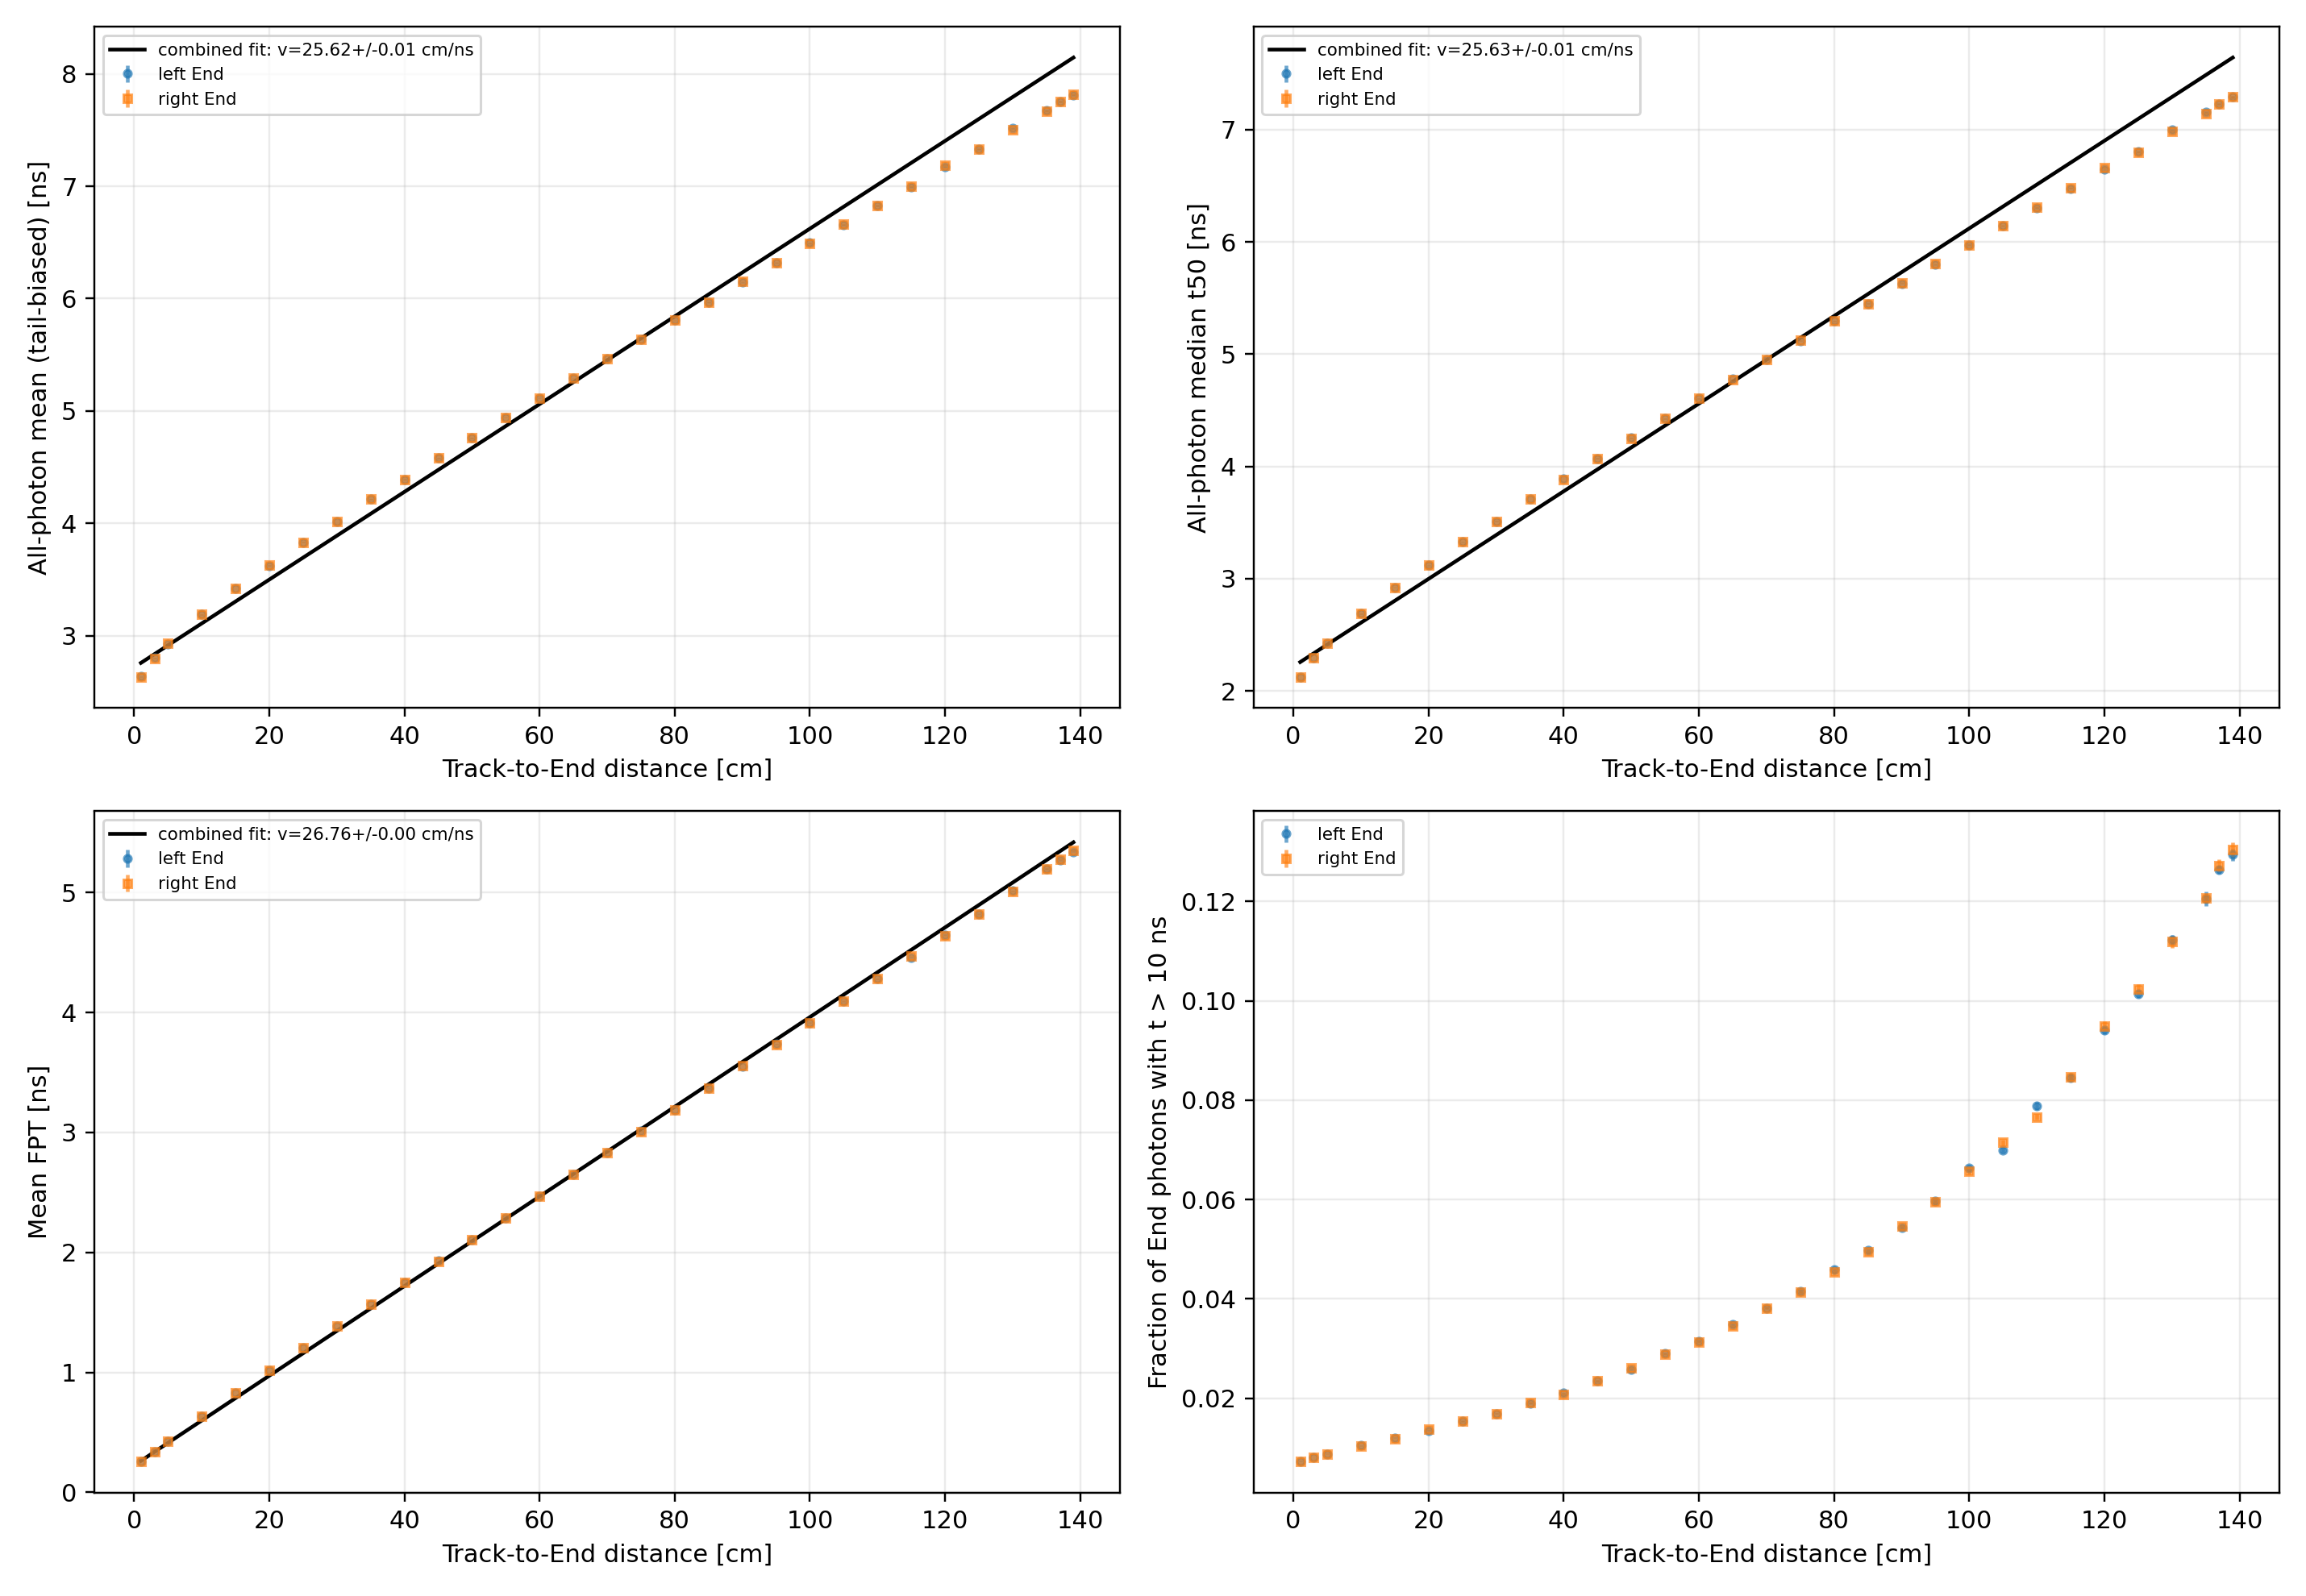
\includegraphics[width=\textwidth]{figs/exec10_velocity_estimators.png}
\column{0.36\textwidth}
\scriptsize\resizebox{\textwidth}{!}{\begin{tabular}{lrr}\toprule
Estimator & slope-derived [cm/ns] & $\chi^2/ndf$ \\ \midrule
all-photon mean & $25.616\pm0.005$ & 3189.9 \\
all-photon $t_{50}$ & $25.625\pm0.005$ & 3615.1 \\
mean FPT & $26.758\pm0.003$ & 1002.6 \\
\bottomrule\end{tabular}}
\begin{alertblock}{Refuted predictions}
Mean FPT is not close to $c/n\simeq19$ cm/ns. The fixed-threshold $f(t>10\,ns)$
increases with distance. Every global line fit is rejected.
\end{alertblock}
\end{columns}

\end{frame}
\begin{frame}{Top readout: analytic timing estimate only}

\centering\small
\begin{tabular}{rrr}\toprule
$x$ [mm] & nearest Top $N_{pe}$ & $\sigma_{t,est}$ [ps] \\ \midrule
-690 & $350.9\pm2.0$ & $59.92\pm0.17$ \\
-650 & $351.0\pm2.0$ & $59.91\pm0.17$ \\
-400 & $411.3\pm2.3$ & $55.35\pm0.16$ \\
+0 & $407.3\pm2.2$ & $55.62\pm0.15$ \\
+400 & $411.4\pm2.4$ & $55.34\pm0.16$ \\
+650 & $350.9\pm2.1$ & $59.93\pm0.18$ \\
+690 & $353.0\pm2.0$ & $59.75\pm0.17$ \\
\bottomrule\end{tabular}
\vspace{0.35cm}
\begin{block}{Definition and scope}
$\sigma_{t,est}=\sqrt{0.7\,\mathrm{ns}\times1.8\,\mathrm{ns}}/\sqrt{N_{pe}}
=1.122\,\mathrm{ns}/\sqrt{N_{pe}}$. This is an analytic orientation,
not a simulated timing resolution; Top has no test-beam counterpart.
\end{block}

\end{frame}
\begin{frame}{Numerical conclusions}

\small\begin{itemize}
 \item At center: End sum $389.6\pm2.1$, nearest Top $407.3\pm2.2$;
       at $x=-690$ mm: End sum $3404.2\pm18.3$, nearest Top $350.9\pm2.0$.
 \item $\lambda_{eff}$: L $33.14\pm0.03$ cm,
       R $33.06\pm0.03$ cm;
       no global time estimator yields an acceptable propagation-velocity fit.
 \item Nearest-Top var/mean: median 24.81, range
       19.14--29.27;
       $F=1+(0.062162\pm0.000107)\langle N_{pe}\rangle$ with
       $\chi^2/ndf=1.76$: Landau-like energy-loss fluctuations dominate.
 \item Intrinsic End $\sigma_{group}$: mean 148.3 ps,
       range 12.1--437.3 ps.
 \item EndTop/End-only timing ratio: $0.756\pm0.016$
       to $0.904\pm0.016$.
 \item Three findings: window-track dip characterized; late-tail drain confirmed;
       complete 86-channel coverage and localization gate validated.
\end{itemize}

\end{frame}
\appendix
\begin{frame}{Backup: validation and gates}

\begin{itemize}
 \item 31/31 ROOT files pass: event IDs 0--1999, matching beam x, aggregate IDs 0--85.
 \item Top localization passes all positions: strict nearest maximum except the documented
       $x\equiv10\pmod{20}$ window-track effect (maximum among nearest two, deficit below 15\%).
 \item At x=300 mm the two candidates differ by only 0.08 sigma and pass as a statistical tie.
 \item MPT checks pass: RINDEX 1.58, yield 10400/MeV, decay 1.8 ns, rise 0.7 ns,
       ABSLENGTH 160 cm, emission peak 408.8 nm.
\end{itemize}

\end{frame}
\begin{frame}{Backup: ID18 impact maps}
\centering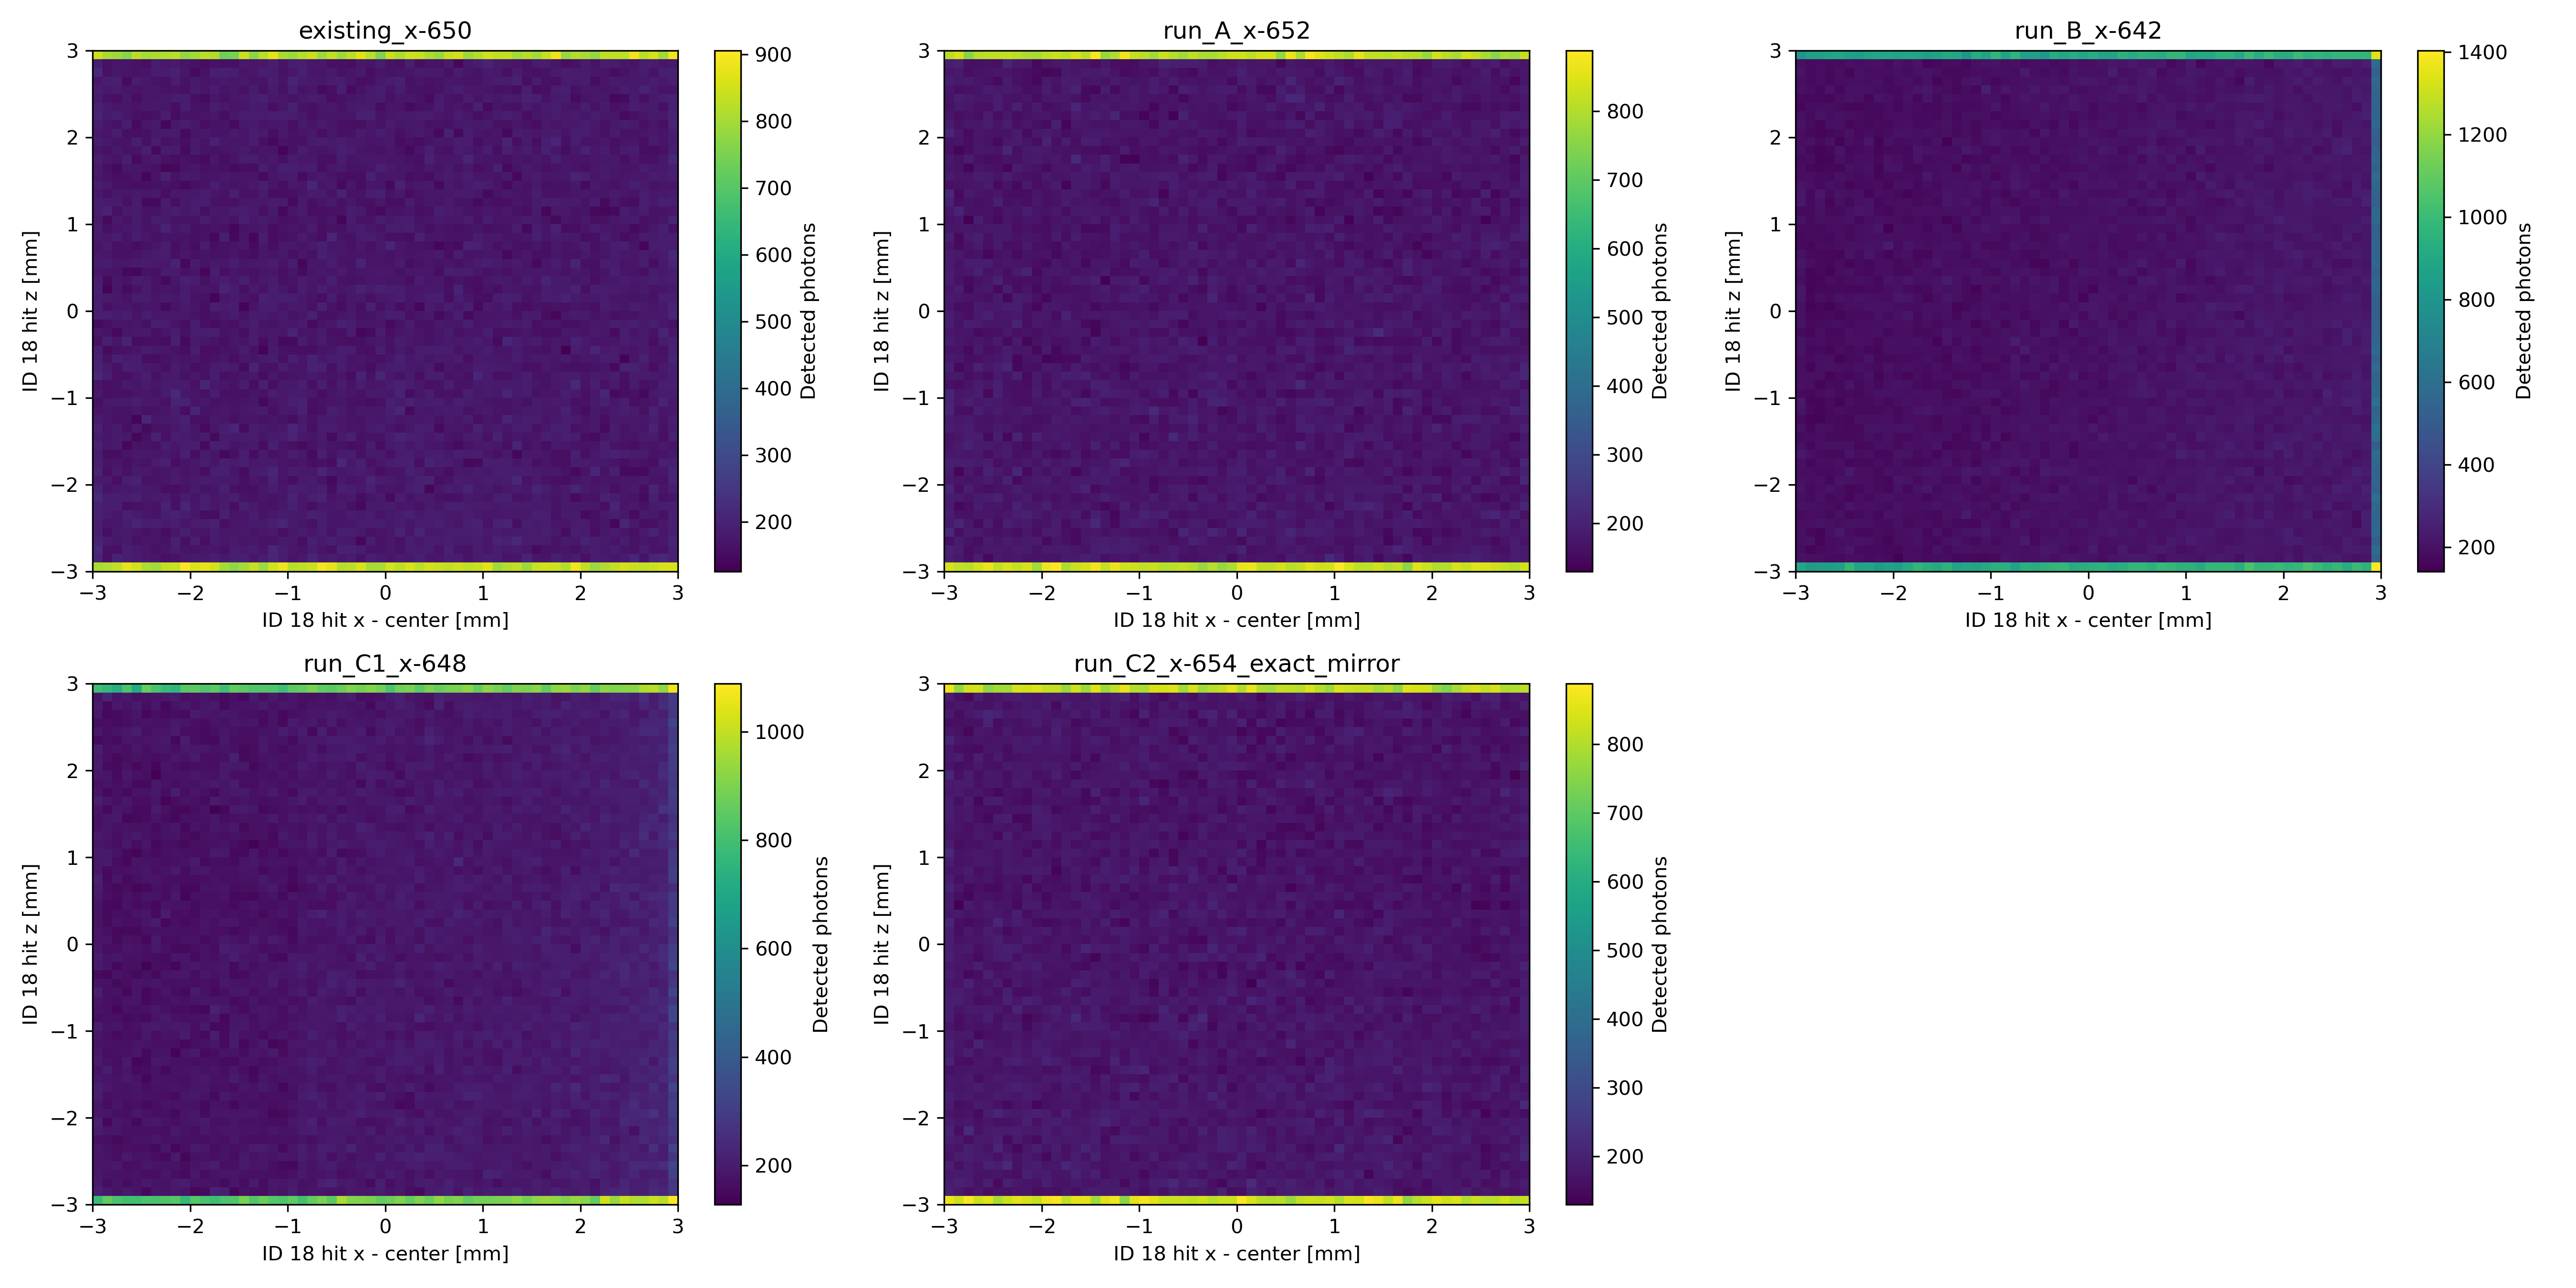
\includegraphics[width=\textwidth,height=0.78\textheight,keepaspectratio]{figs/exec08b_id18_impact_maps.png}
\end{frame}
\begin{frame}{Backup: timing methodology}

\begin{itemize}
 \item SUM4 groups: \{0..3\}, \{4..7\}, \{8..11\}, \{12..15\}.
 \item Single-PE response: normalized 0.5/5 ns double exponential.
 \item Absolute leading-edge threshold: 4 PE equivalent.
 \item Estimator: $\sigma(\Delta T_{AB})/\sqrt{2}$.
 \item \texttt{HOOK\_WALK}: pending; no time-walk correction exists or was invented.
 \item EXEC\_09 anti-artifact audit verifies common threshold, pulse, t=0 and estimator.
\end{itemize}

\end{frame}
\begin{frame}{Backup: glossary}

\scriptsize\begin{description}
 \item[HOOK\_WALK] Reserved insertion point for future leading-edge time-walk correction.
 Fixed 4-PE threshold means larger pulses cross earlier; no correction is applied
 in any campaign (\texttt{congruent\_sum4\_timing.C:305--315}).
 \item[FPT] First photon time: first detected photon in an event for the stated channel/group.
 \item[SUM4] Analog sum of four SiPMs: \{0--3\}, \{4--7\}, \{8--11\}, \{12--15\}.
 \item[(exact geometry)] Nearest geometric SiPM agrees with the maximum, or is covered by
 the documented window-track exception; x=300 mm is explicitly a statistical tie.
 \item[Temporal density] Absolute plots are entries/event/ns; normalized plots integrate to one
 and compare shape only.
 \item[Central 24 mm pair] The sole pitch exception is $-12/+12$ mm because 1384 mm is not
 divisible by 20 mm.
 \item[Intrinsic sigma] Excludes SPTR and electronics jitter; the hardware 88 ps value is not
 directly comparable.
\end{description}

\end{frame}
\begin{frame}{Backup: EndTop versus End-only tail audit}
\centering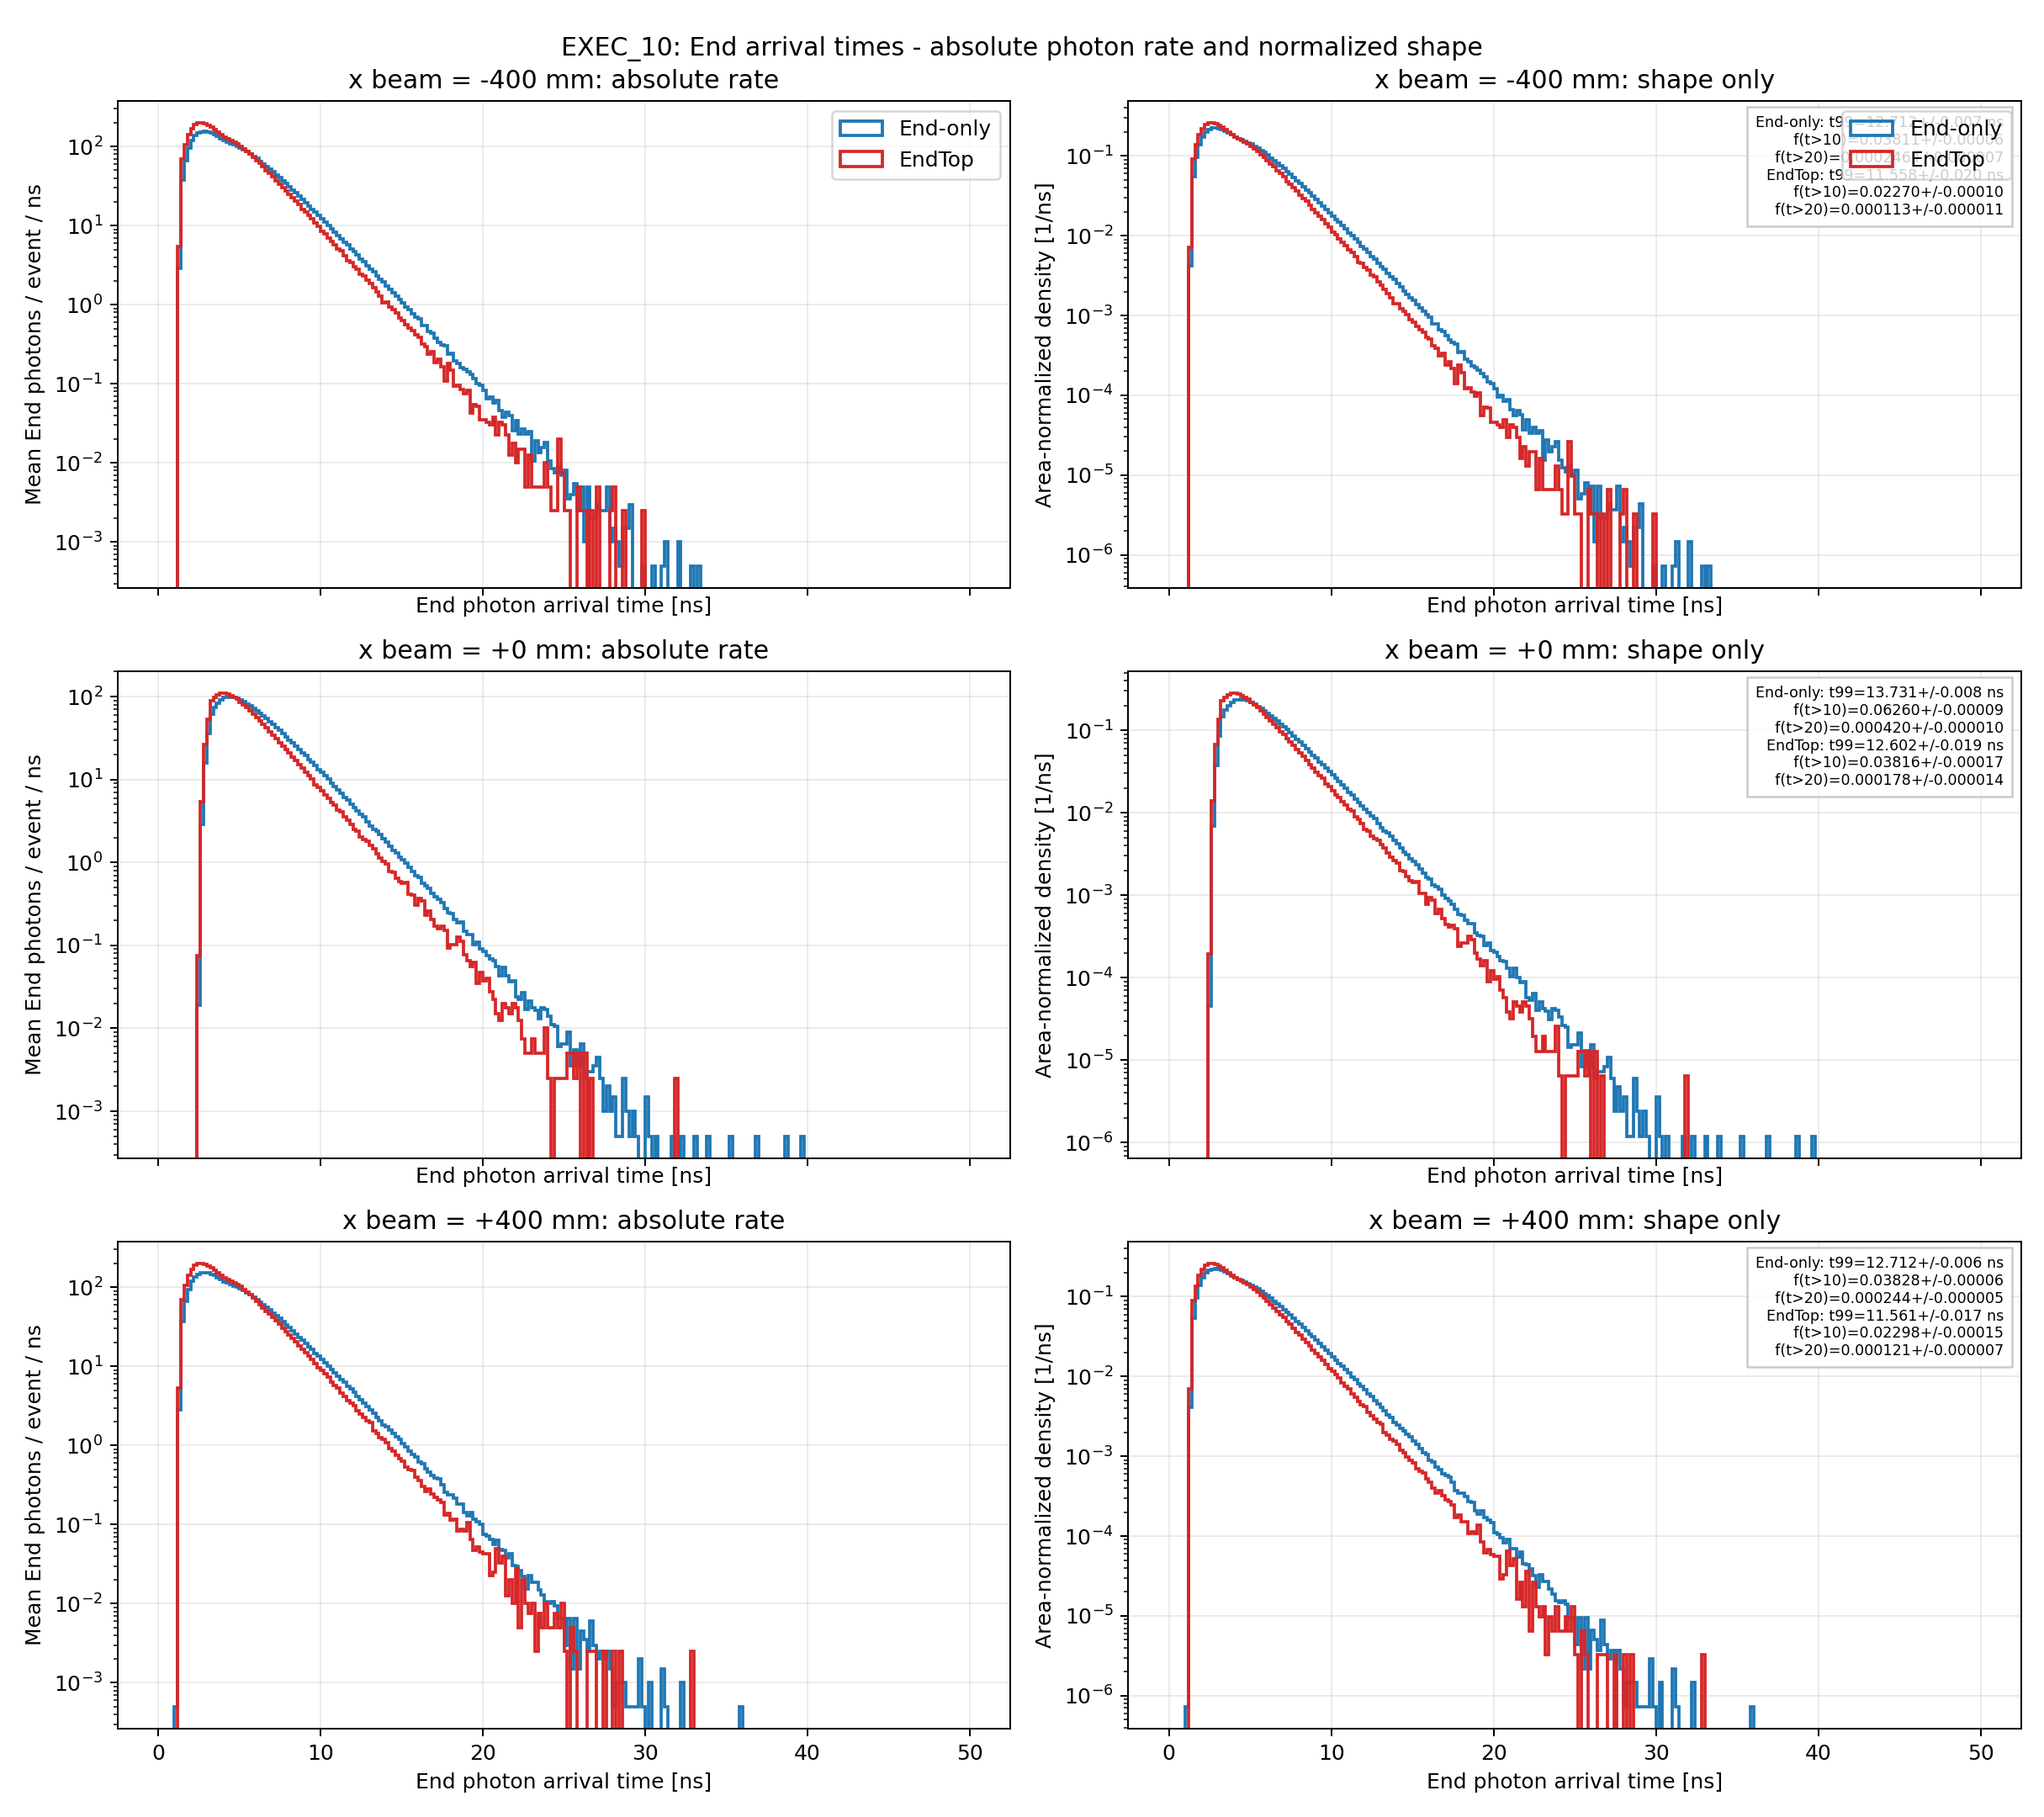
\includegraphics[width=\textwidth,height=0.78\textheight,keepaspectratio]{figs/exec09_tail_comparison.png}
\end{frame}
\end{document}
